\documentclass{rapportENSCP}
\usepackage{lipsum}
\usepackage{tabularx} 
\title{Rapport Stage Ouvrier- Template} %Thanks for Rapport
\begin{document}

%----------- Informations du rapport ---------

\logoentreprise{logos/logoRewake.jpg}

\titre{Rapport de stage ouvrier} % Titre du fichier

\mention{Stage de découverte de l'entreprise} % Nom de la Mention
%\trigrammemention{Master IA} % Pour le bas de la page
\master{Cycle Ingénieur} % Nom du master
%\filiere{Filière Management de projet et Transformation} % Nom de la filière

\eleve{Alban Laborde-Laulhé}

\dates{7 août 2024 - 30 août 2024}

% Informations tuteurs écoles
\tuteurecole{
    \textsc{Philippe Vernazobres} \\
    philippe.vernazobres@chimieparistech.psl.eu
} 

\tuteurentreprise{
    \textsc{Paul Forget} \\
    paul@rewake.fr
}

%----------- Initialisation -------------------
        
\fairemarges %Afficher les marges
\fairepagedegarde %Créer la page de garde

%----------- Abstract -------------------
%\vspace*{\stretch{1}}
%\begin{center}
%	\begin{abstract}
%        \lipsum[1]
%        \rule{\linewidth}{0.2 mm} \\[0.4 cm]
%        \begin{center}\textbf{Summary :}\end{center} 
%        \lipsum[2]
%    \end{abstract}
%\end{center}
%\vspace*{\stretch{1}}
%\newpage

%------------ Table des matières ----------------

\tabledematieres % Créer la table de matières

%------------ Corps du rapport ----------------


%------------ Introduction ----------------

\section{Executive summary} 
% Effacer les lignes suivantes et écrire le texte souhaité
Ce rapport présente une synthèse des activités réalisées lors de mon stage au sein de Rewake, une jeune startup spécialisée dans le reconditionnement de matériel de laboratoire. Ce stage m’a offert une immersion complète dans un environnement entrepreneurial dynamique, combinant des tâches à la fois techniques, logistiques et commerciales. L’entreprise, dont le modèle s’inscrit pleinement dans une démarche d’économie circulaire, vise à donner une seconde vie à des équipements scientifiques en les récupérant, reconditionnant, puis en les revendant à des laboratoires à moindre coût.

Au cours de ces quatre semaines, j’ai principalement travaillé dans l’entrepôt de Montreuil, où les activités de réception, de réparation et de reconditionnement des équipements se déroulaient. Ces travaux incluaient le démontage et la remise en état de divers instruments, la prise de photographies commerciales pour la plateforme en ligne, et la gestion des stocks à travers la mise à jour des inventaires. Mon rôle s’est progressivement élargi pour inclure des tâches de support aux dirigeants, notamment à travers le profilage de clients potentiels et l'optimisation des bases de données.

L’expérience chez Rewake m’a également permis d’appréhender les enjeux liés à la sécurité au travail dans un contexte industriel. L’utilisation d’équipements lourds et de produits chimiques requiert des mesures de prévention strictes, et Rewake a mis en place des protocoles de sécurité pour assurer la protection des employés. Le port d’équipements de protection individuelle (EPI) est obligatoire, accompagné de formations sur la manipulation des charges et l’utilisation des produits dangereux.

Du point de vue de la gestion des ressources humaines, Rewake fonctionne avec une structure simple où la polyvalence est un atout majeur. La petite taille de l’entreprise favorise un mode de gestion par ajustement mutuel, où les employés échangent constamment sur leurs tâches pour garantir une efficacité optimale. Les dirigeants, très impliqués dans les opérations quotidiennes, apportent une supervision directe lorsque nécessaire, tout en laissant une large autonomie aux employés dans la réalisation de leurs missions.

Ce stage m’a permis d’acquérir des compétences pratiques et techniques variées, tout en me sensibilisant aux enjeux du développement durable dans un secteur industriel. Rewake, bien qu’étant encore en phase de développement, affiche un fort potentiel de croissance, notamment grâce à son engagement en faveur de l’économie circulaire et de la durabilité environnementale. Les défis liés à l’optimisation des pratiques internes et à la gestion des ressources apparaissent comme des opportunités de progression pour cette startup ambitieuse.

En conclusion, ce stage m’a non seulement permis de développer des compétences techniques et organisationnelles, mais il a également renforcé mon intérêt pour l’innovation au service du développement durable dans le secteur scientifique et industriel.

\section{Remerciements}
A Monsieur Philippe Vernazobres, Responsable du Département "Management, Langues et Culture" et de la Cellule "Accompagnement du Projet professionnel et Stages",
Merci pour votre aide et vos conseils précieux.

A Madame Mariane Ighilahriz, Responsable relations entreprises au sein de Chimie Paris. Merci pour votre accompagnement dans ma recherche de stage et d'avoir fait partager tant d'opportunités à notre promotion.

A Monsieur Paul Forget, CEO de Rewake et mon tuteur de stage. Je tiens à vous exprimer toute ma gratitude pour m'avoir offert l'opportunité d'intégrer votre entreprise. Votre soutien, votre bienveillance,les explication détaillées que vous m'avez apportées ainsi que la confiance accordée ont été pour moi des éléments moteurs dans la réussite de ce stage.J'ai pu ainsi en participant aux activités de votre équipe acquérir une compréhension précieuse des défis managériaux et enjeux propres aux entreprises libérales.Pour tout ceci je vous suis infiniment reconnaissant.

A Alban, Antoine, Franck et à toute l'équipe de Rewake. Grand merci pour votre accueil et votre appui. Vous m'avez conseillé et guidé chaque jour.Je garderai le souvenir de votre dynamisme et de votre gentillesse.



\section{Place de l’unité et du service dans l’entreprise}
\label{sec:section2}

Rewake est une jeune startup avec un effectif limité vis-à-vis de la pluralité des travaux à réaliser. Son organisation s’apparente à la structure simple telle que décrite dans l’œuvre de Mintzberg. Les salariés font partie d'une unité fonctionnelle unique prenant en charge l'ensemble du cycle achat-reconditionnement-revente du matériel de laboratoire. Ils effectuent autant les tâches opérationnelles que le support logistique nécessaire au fonctionnement de l'entreprise. 

Le lien hiérarchique entre les salariés s'apparente au concept \emph{Staff and Line}. En effet, un lien de conseil s'établit entre les employés exécutant différentes tâches. Par exemple, lors de la préparation d'un produit, celui responsable du marketing va indiquer à l'employé en charge du nettoyage les parties à privilégier car importantes aux yeux du client. 

\section{Structuration du service}
\label{sec:section3}
L'entreprise n'est constituée que d'un seul service, celui-ci englobant l'ensemble des composantes de l'organisation de l'entreprise. Les employés sont invités à participer à chacune d'entre elles en fonction des besoins du moment. La séparation des unités de l’entreprise est alors plus marquée par le lieu du travail que par son personnel.

\noindent Rewake dispose ainsi de deux locaux :
\begin{itemize}
    \item 5 postes PC à Station F (un espace dédié l’incubation de startup)
    \item Un espace de bureaux et un entrepôt à Montreuil
\end{itemize}
\vspace{0.4cm}

Néanmoins, Rewake dispose tout de même d'un organigramme d'entreprise, précisant la tâche principale de chaque salarié même s'il n'y est pas limité.

\begin{figure}[H]
    \centering
    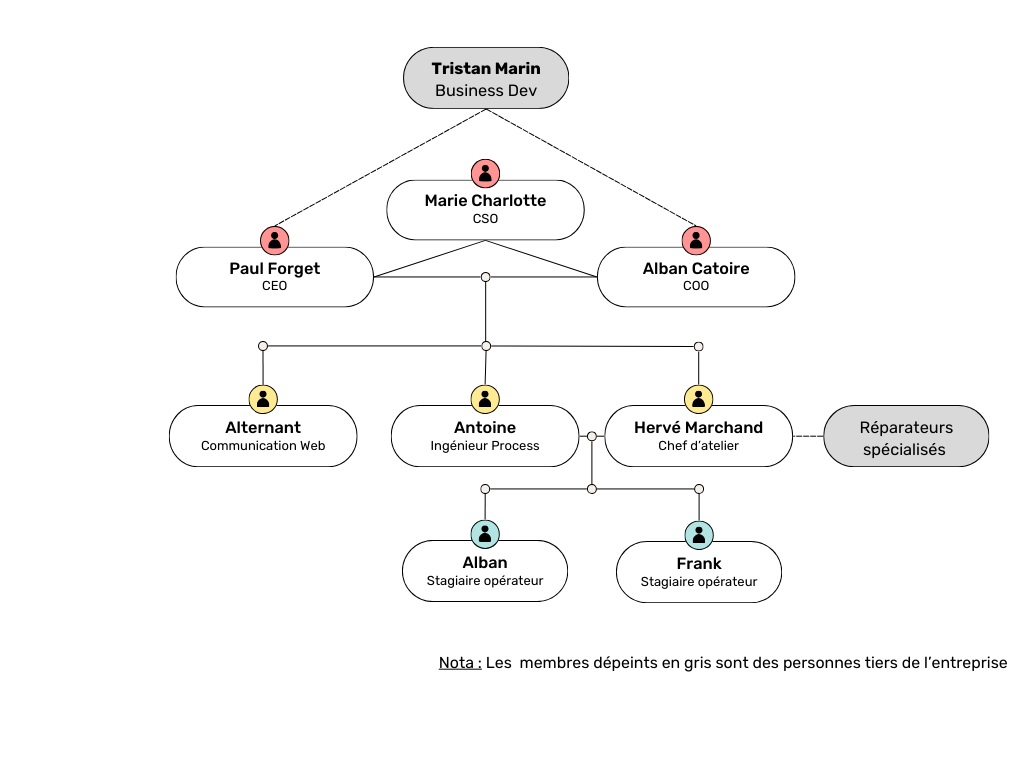
\includegraphics[width = 1\textwidth]{figures/orgaRewake.png}
    \caption{Organigramme de l'entreprise}
    \label{fig:organigramme}
\end{figure}

\subsection{Sommet stratégique}

On repère bien dans la figure \ref{fig:organigramme} l'imposant sommet stratégique propre aux structures simples. Composé de trois membres : Alban Catoire et Paul Forget respectivement CEO et COO possédant chacun 50\% des parts de la startup, et Marie Charlotte CSO, conseillère, s'assurant de la bonne croissance de l'entreprise. 

Il s'agit du seul pôle dont les membres sont clairement définis. Ceux-ci s'occupent de la direction stratégique de l'entreprise et de ses finances.


\subsection{Centre opérationnel de l'entreprise}
Rewake propose une offre de matériel de laboratoire reconditionné. Elle est crée grâce aux travaux réalisés dans l'entrepôt de Montreuil. Ici les employés s'occupent de réceptionner les livraisons de matériel de laboratoire usagé, d'évaluer leur état puis de réaliser le reconditionnement fonctionnel et esthétique du matériel avant de le préparer pour sa future expédition.

Ce lieu est le coeur de la production opérationnelle de Rewake, conçu comme une unité de projet dédiée au reconditionnement. Il s'agit d'un espace de travail modulaire au sein duquel les opérateurs sont libres de déplacer les établis et les outils de travail en fonction des besoins de leur tâche.

Cependant avec le développement de l'entreprise, il est prévu de transformer cette unité de projet en sous-unités de produits grâce au développement de protocoles de reconditionnement par type de produit permettant aux opérateurs de ne traiter qu'un type de matériel dans un établi défini.

\subsection{Support logistique de l'entreprise}
La chaîne logistique de Rewake répond à une demande s'inscrivant dans un marché d'économie circulaire. Ainsi, pour assurer la fluidité de la production, Rewake doit à la fois démarcher de potentiels acheteurs de produits de seconde main mais également des vendeurs de matériel d'occasion, usagé ou déclassé. 

Ce travail de support est réalisé dans les bureaux de Montreuil ou à Station F par les deux dirigeants comme leurs employés. Le support logistique de l'entreprise s'occupe également de contacter des réparateurs spécialisés nécessaires au reconditionnement de certains appareils mais aussi de répondre aux doléances du centre opérationnel en s'occupant de lui fournir le matériel dont il a besoin. 

\subsection{Technostructure}
La technostructure de Rewake est en premier lieu incarnée par son ingénieur process, responsable du développement des techniques de reconditionnement de l'entreprise et de l'aménagement de l'entrepôt, qui sert à la fois de lieu de stockage et d'atelier de réparation. Cet ingénieur se renseigne sur le fonctionnement des appareils acquis par l'entreprise et prépare des protocoles standardisés de réparation.

Par ailleurs, Rewake dispose d'une plate-forme commerciale en ligne encore en phase de développement lors de la période de mon stage. Son développement est pris en charge par une seconde technostructure incarnée par le consultant web, les deux dirigeants ainsi que, dans une moindre mesure, les autres employés. Cette unité s'occupe, d'une part, de l'esthétique et de l'ergonomie de la plate-forme en ligne pour les clients, et d'autre part, de la structuration de l'inventaire des articles mis en vente, à travers une base de données en cours de création durant mon mois de stage.

\subsection{Encadrement et exercice du pouvoir}
L'encadrement est majoritairement assuré directement par les deux dirigeants, qui proposent les tâches à réaliser en fonction des priorités du moment. Par exemple, il a été demandé à un employé, initialement chargé de mettre à jour l'inventaire, de se concentrer désormais sur le profilage de personnalités proches des domaines d'activité de l'entreprise, en prévision d'un salon à venir. Cela illustre l'exercice parfois "ad-hoc" du pouvoir et la capacité de toute l'équipe à changer de tâche rapidement et efficacement.

De plus, durant mon stage, ma ligne hiérarchique s'organisait en deux niveaux : je devais en premier lieu assister l'ingénieur process dans ses tâches, et en second lieu, répondre aux demandes des deux dirigeants si l'ingénieur n'avait rien à me proposer.


\section{Contenu du travail}

Ma période de travail était répartie sur 5 jours, de 9h30 à 17h avec une pause d'une heure entre midi et deux.  Le travail effectué lors de ces 4 semaines de stage fut plus que varié. Les différentes tâches expérimentées sont reparties en deux grandes catégories : les travaux manuels effectués à l'entrepôt de Montreuil et les travaux de bureautique effectués aux bureaux de Montreuil et à Station F.

\subsection{Travaux à l'entrepôt}
Ces travaux sont centrés sur le reconditionnement de matériel de laboratoire, qui constitue l'activité principale de l'entreprise, mais incluent également la préparation à leur commercialisation. Cela comprend l'acquisition des données techniques des équipements réparés ainsi que la prise de photographies commerciales destinées à leur mise en vente.

L'équipe principale dans l'entrepôt lors de mon stage était composée d'un ingénieur process, de moi-même et d'un second stagiaire ouvrier. Les deux dirigeants participaient également aux tâches lorsque cela était nécessaire et supervisaient la conformité des travaux effectués avec les objectifs de l'entreprise.

\subsubsection{Nettoyage esthétique de matériel de laboratoire}
\label{subsubsec:paillasse}
Au début de mon stage, Rewake a reçu une grande quantité de paillasses de laboratoire usagées. Nous avons également nettoyé une machine à glace et un réfrigérateur. Mon travail consistait à :

\begin{itemize}
    \item M'assurer que les paillasses ne présentaient pas de défauts trop importants (planche fracturée, table mal ajustée, pièce manquante, etc.).
    \item Retirer les étiquettes, rubans adhésifs et autres éléments ajoutés par l'ancien propriétaire.
    \item Nettoyer les paillasses à l'eau et à la lessive pour leur donner un état "comme neuf".
\end{itemize}

Cette tâche était effectuée en coordination avec le second stagiaire ouvrier de l'entreprise, chaque paillasse étant nettoyée à deux. Elle était supervisée par l'ingénieur process ainsi que par le CEO.

Le matériel utilisé pour réaliser cette activité était le suivant :
\begin{itemize}
    \item Éponges dures, fines et magiques pour le nettoyage des taches.
    \item Eau et lessive de chantier.
    \item Acétone, nécessaire à la suppression des étiquettes, rubans adhésifs et traces de peinture.
    \item Tournevis pour retirer les vis dangereuses.
    \item Tournevis plat et pince pour retirer les joints et les taches tenaces.
\end{itemize}

La principale difficulté rencontrée était de savoir à quel moment le travail sur une paillasse pouvait être considéré comme terminé. En effet, de nombreuses traces sur les paillasses usagées s'enlevaient très difficilement, voire pas du tout, malgré des efforts répétés. Cela soulevait la question de savoir s'il fallait persister de longues minutes sur une trace peu visible ou, à l'inverse, considérer le travail terminé malgré ces défauts.

Ainsi, en l'absence de description précise du résultat attendu après le nettoyage, la fin du travail était déterminée par consensus entre mon coéquipier et moi-même, avec, en cas de doute, un contre-avis de l'ingénieur process.

Cette difficulté a été exprimée à la direction, qui en a conscience. Elle a admis qu'à terme, l'entreprise publierait des protocoles détaillés à destination de ses employés pour ce type de tâche.

\subsubsection{Reconditionnement de matériel de laboratoire}
\label{subsubsec:multiposte}
Lors de mon stage j'ai pu assister l'ingénieur process au reconditionnement d'une machine de laboratoire : un agitateur magnétique multiposte dont la courroie était défectueuse (voir figure \ref{fig:agitateur}).

\begin{figure}[H]
    \centering
    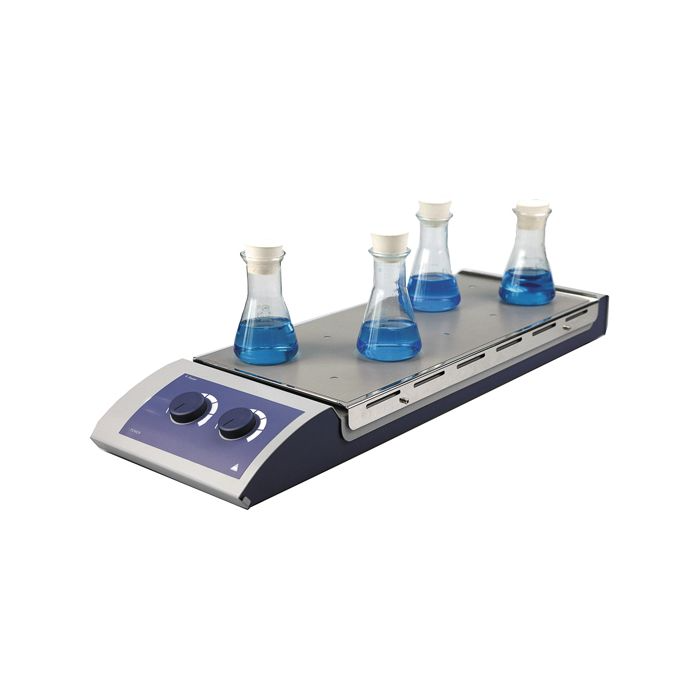
\includegraphics[width = 0.5\textwidth]{figures/agitateur.png}
    \caption{Illustration d'un agitateur multiposte en état de marche}
    \label{fig:agitateur}
\end{figure}

Il s'agissait de remplacer l'ancienne courroie par une nouvelle commandée pour l'occasion. Celle-ci étant vendue sous la forme d'une bobine de fil plastique, il fallait en couper une longueur idoine puis en faire une solide courroie circulaire en soudant les deux bouts au fer à souder afin de remplacer l'ancienne. Pour cela l'ingénieur process avait au préalable conçu deux pièces imprimées en 3D permettant de loger les extrémités du fil pendant la soudure afin d'assurer que la reliure soit la plus solide possible. Une fois la courroie fabriquée il a suffi de la tendre sur les roues de l'appareil pour que l'agitateur soit de nouveaux capable de fonctionner correctement.

Cette expérience m'a permis d'entrevoir les différentes étapes propres au reconditionnement d'un matériel spécifique :

\begin{itemize}
    \item L'évaluation des dommages et la viabilité à les réparer : ici l'agitateur fonctionnait parfaitement mis à part la courroie qui était rompue.
    \item La conception d'outils efficaces propres aux travaux de reconditionnement : ici les pièces conçues puis imprimées en 3D, preuves de l'absence d'outil efficace de réparation déjà présent à la vente.
    \item La réalisation du reconditionnement en changeant la pièce défectueuse par une pièce identique.
    \item La vérification de l'appareil reconditionné, en testant son fonctionnement/état de marche ainsi qu'en vérifiant la solidité de la nouvelle courroie.
\end{itemize}


\subsubsection{Prise de photographies à destination commerciale}
Afin de publier les différents articles reconditionnés sur la plate-forme commerciale en ligne de Rewake, il est nécessaire de les prendre en photos sous différentes prises de vue afin de permettre au client de visualiser dans sa globalité le produit auquel il s'intéresse.

\begin{figure}[H]
    \centering
    \begin{minipage}[c]{0.23\textwidth}
        \centering
        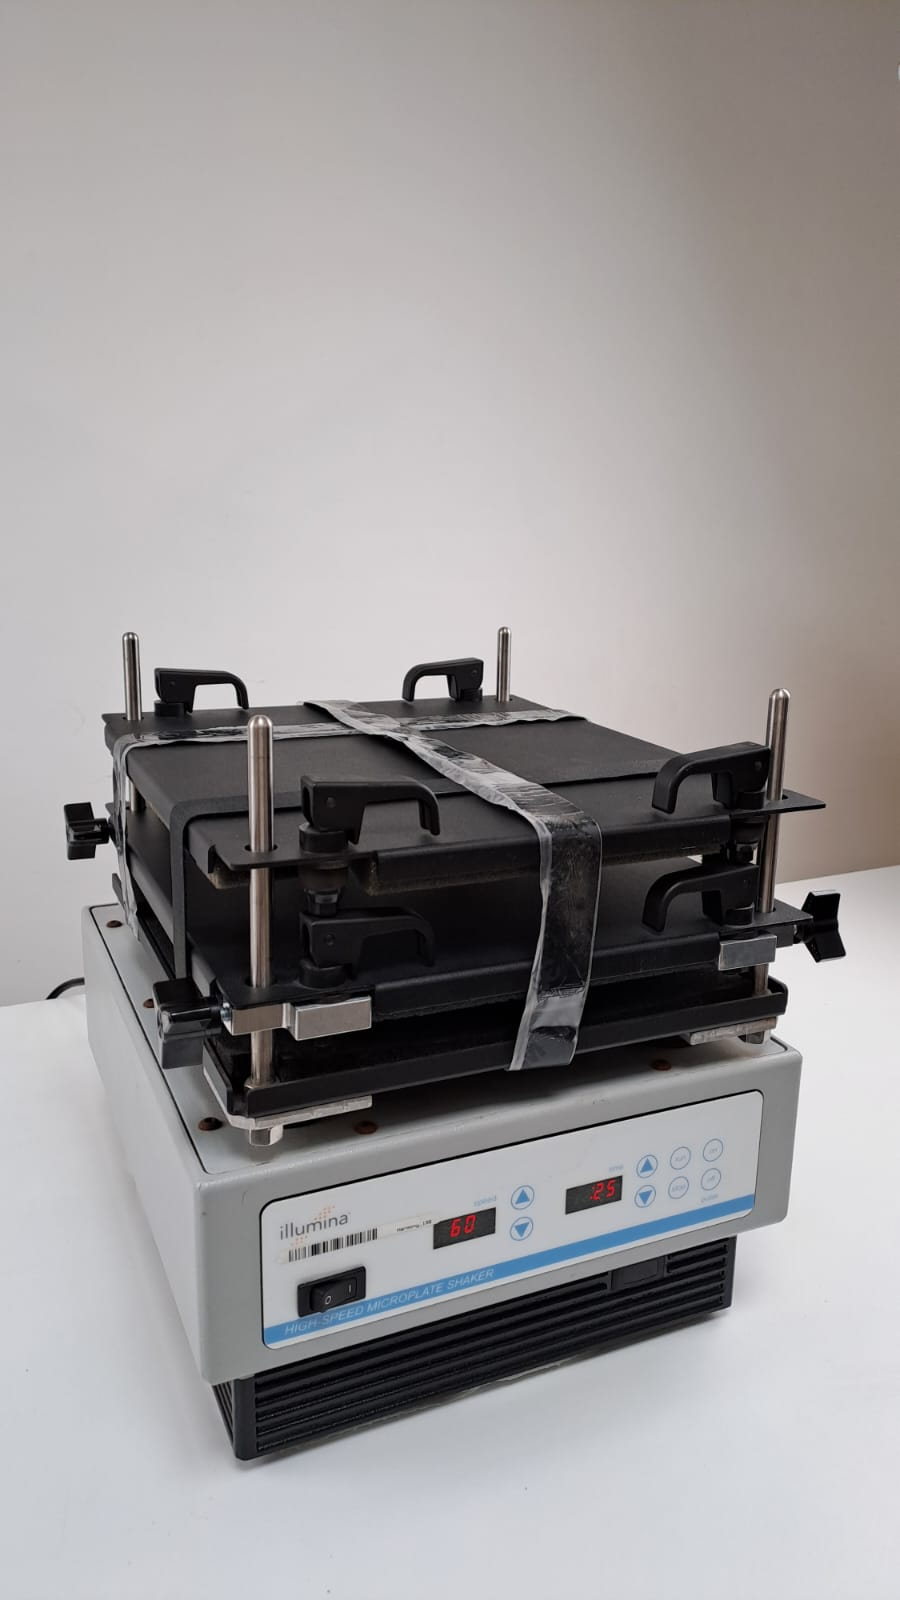
\includegraphics[width=\textwidth]{figures/agitatruc.jpg}
    \end{minipage}
    \hspace{0.2cm} % Espace horizontal entre les images
    \begin{minipage}[c]{0.4\textwidth}
        \centering
        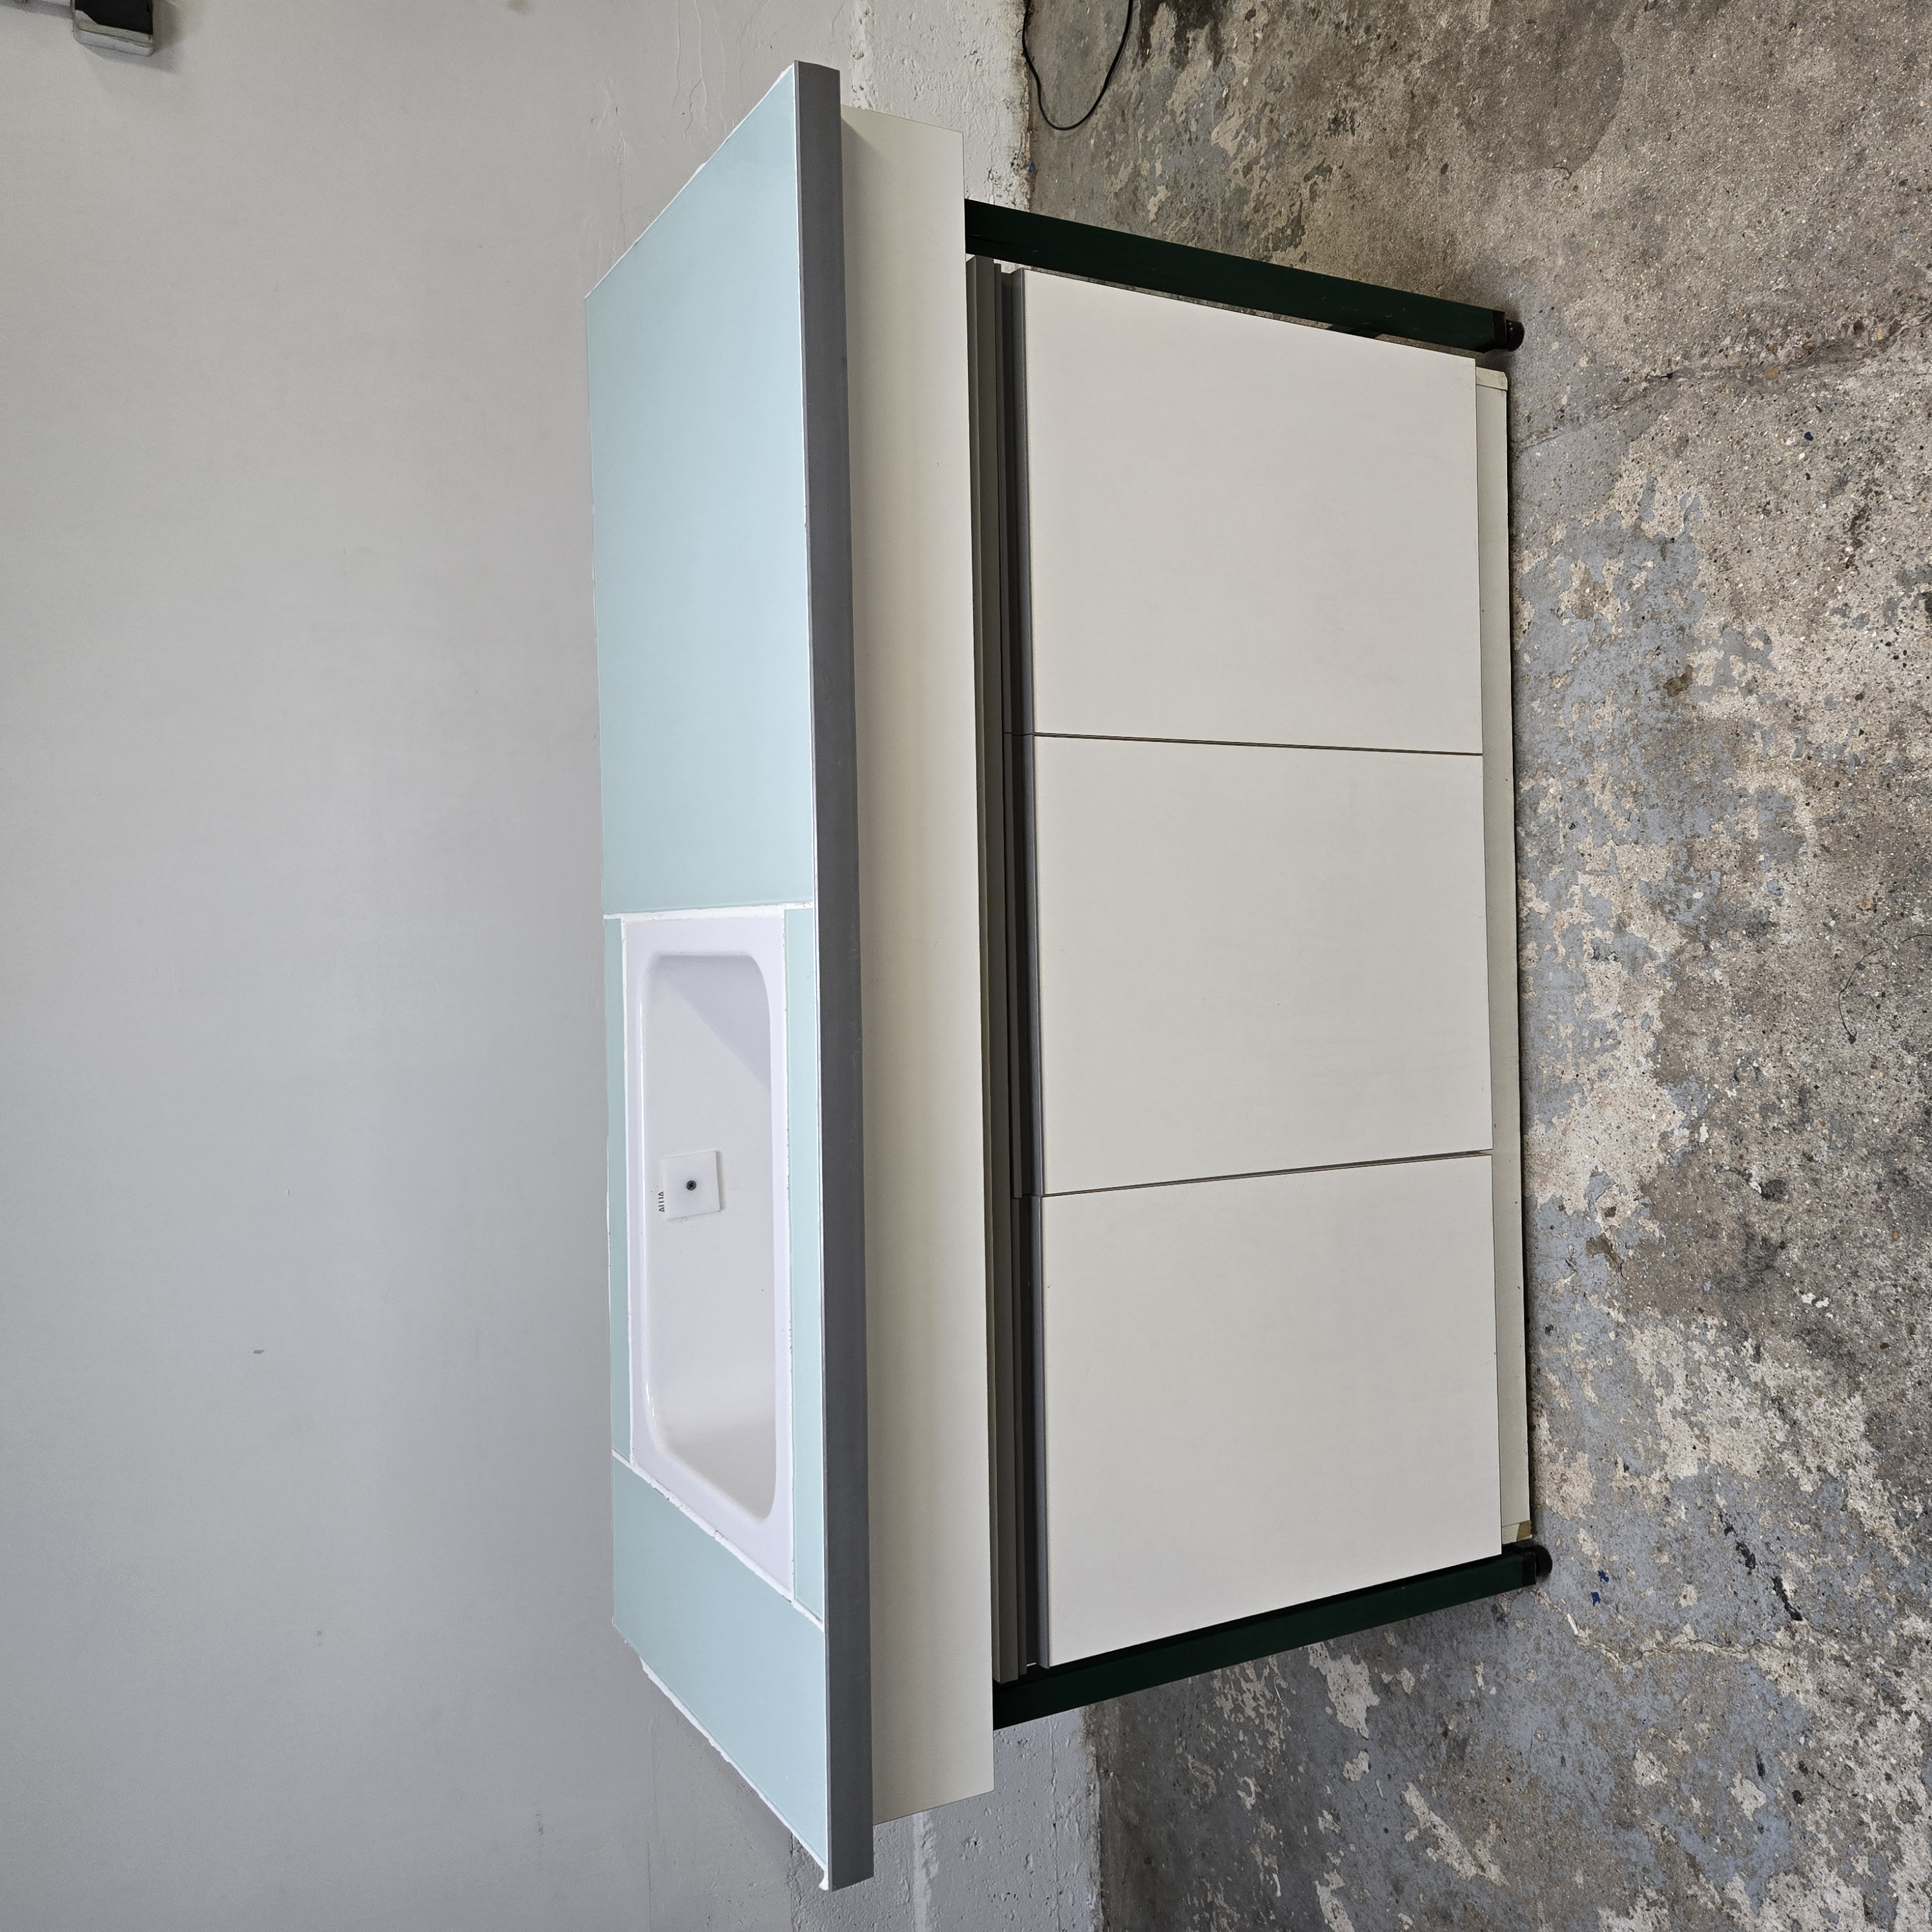
\includegraphics[width=\textwidth, angle=270]{figures/paillasse.jpg}
    \end{minipage}
    \hspace{0.2cm} % Espace horizontal entre les images
    \begin{minipage}[c]{0.23\textwidth}
        \centering
        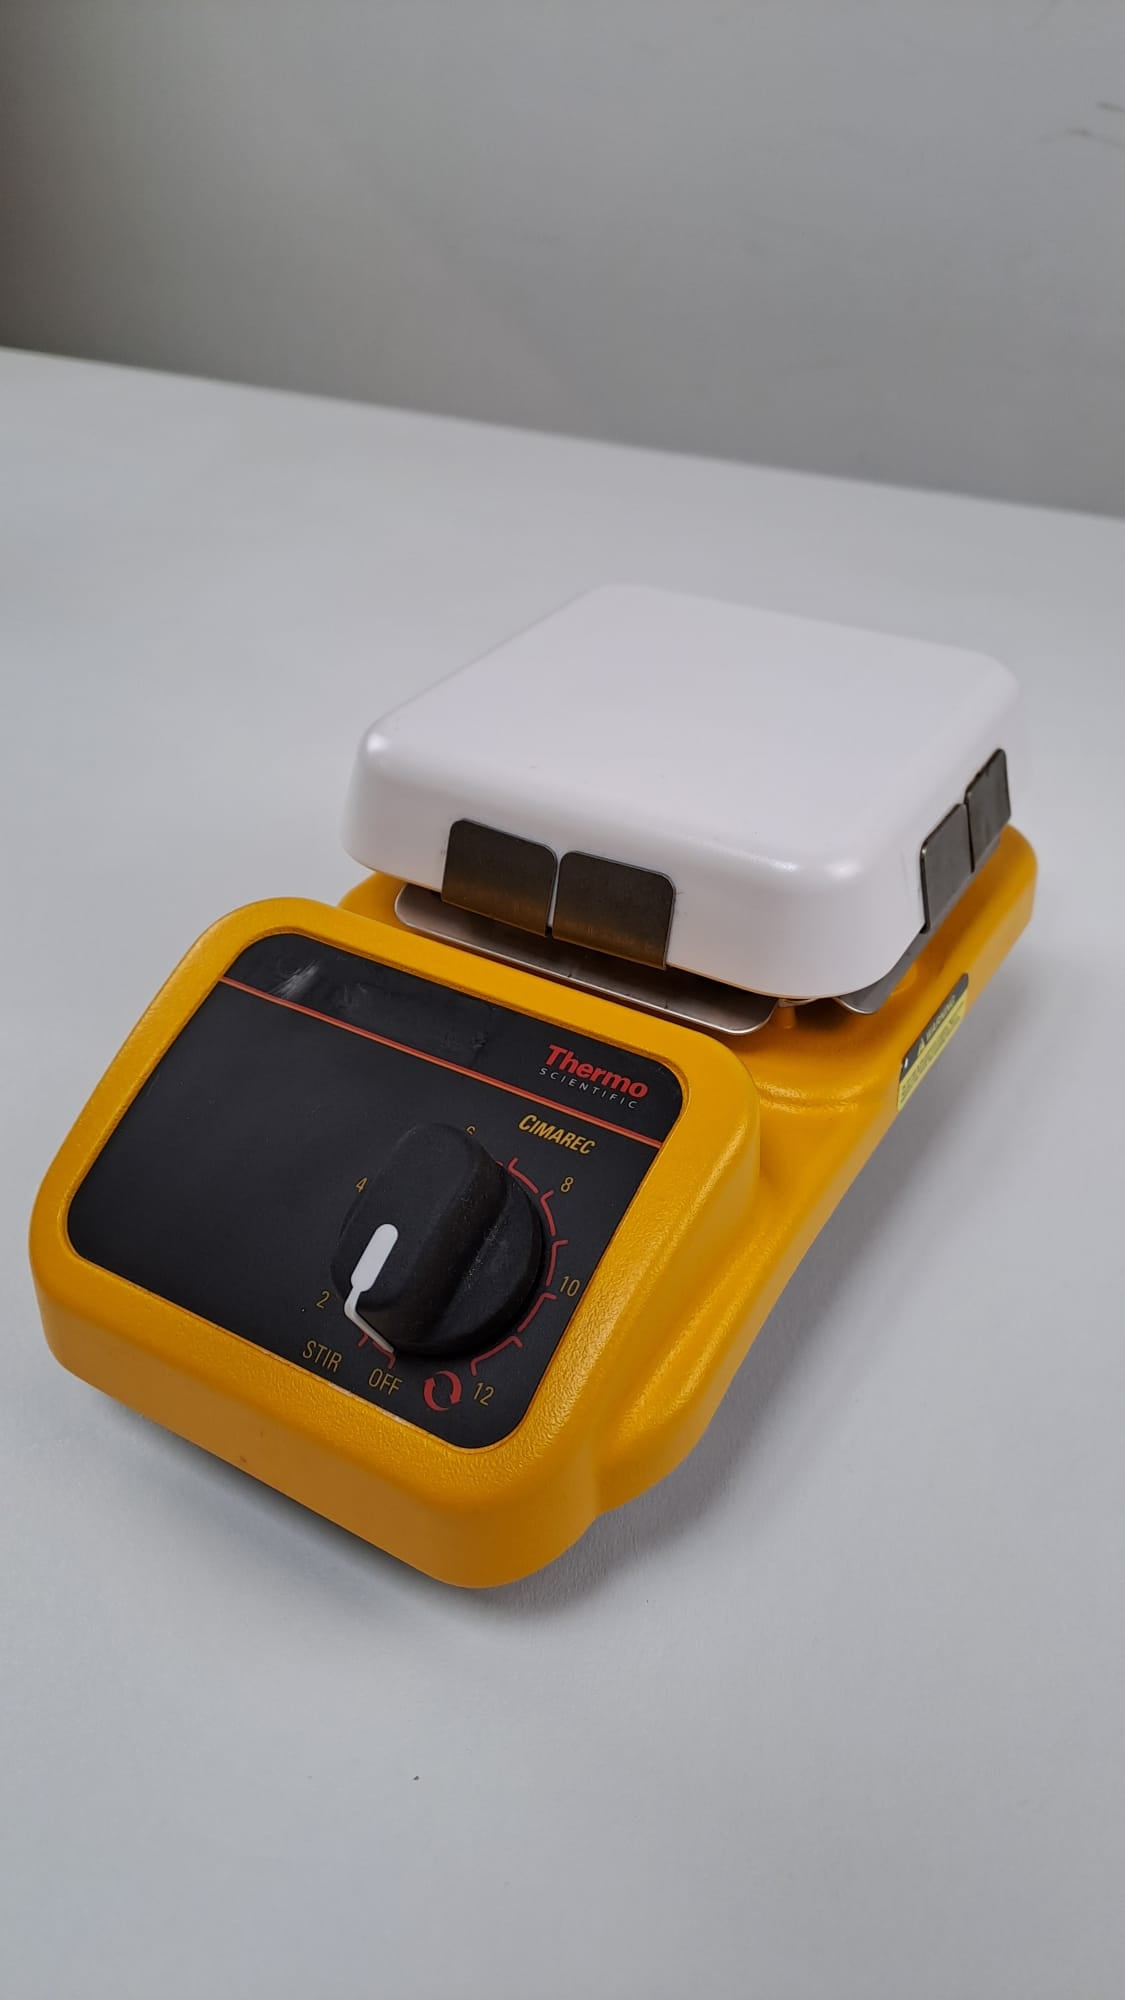
\includegraphics[width=\textwidth]{figures/agitateur2.jpg}
    \end{minipage}
    \caption{Exemple de photographies prises à destination du site web}
    \label{fig:photobrut}
\end{figure}


Pour cela, avec mon coéquipier stagiaire ouvrier, nous déplacions le matériel prêt à la vente dans un petit studio photo disposé dans le hangar. Pour chaque produit une photo de face, de profil et de dos était prises.

Il était nécessaire de considérer quels éléments du produit pourraient intéresser le client et donc quelles prises en surcroît des trois premières photographies seraient intéressantes à prendre. 

\begin{figure}[H]
    \centering
    \begin{minipage}[c]{0.27\textwidth}
        \centering
        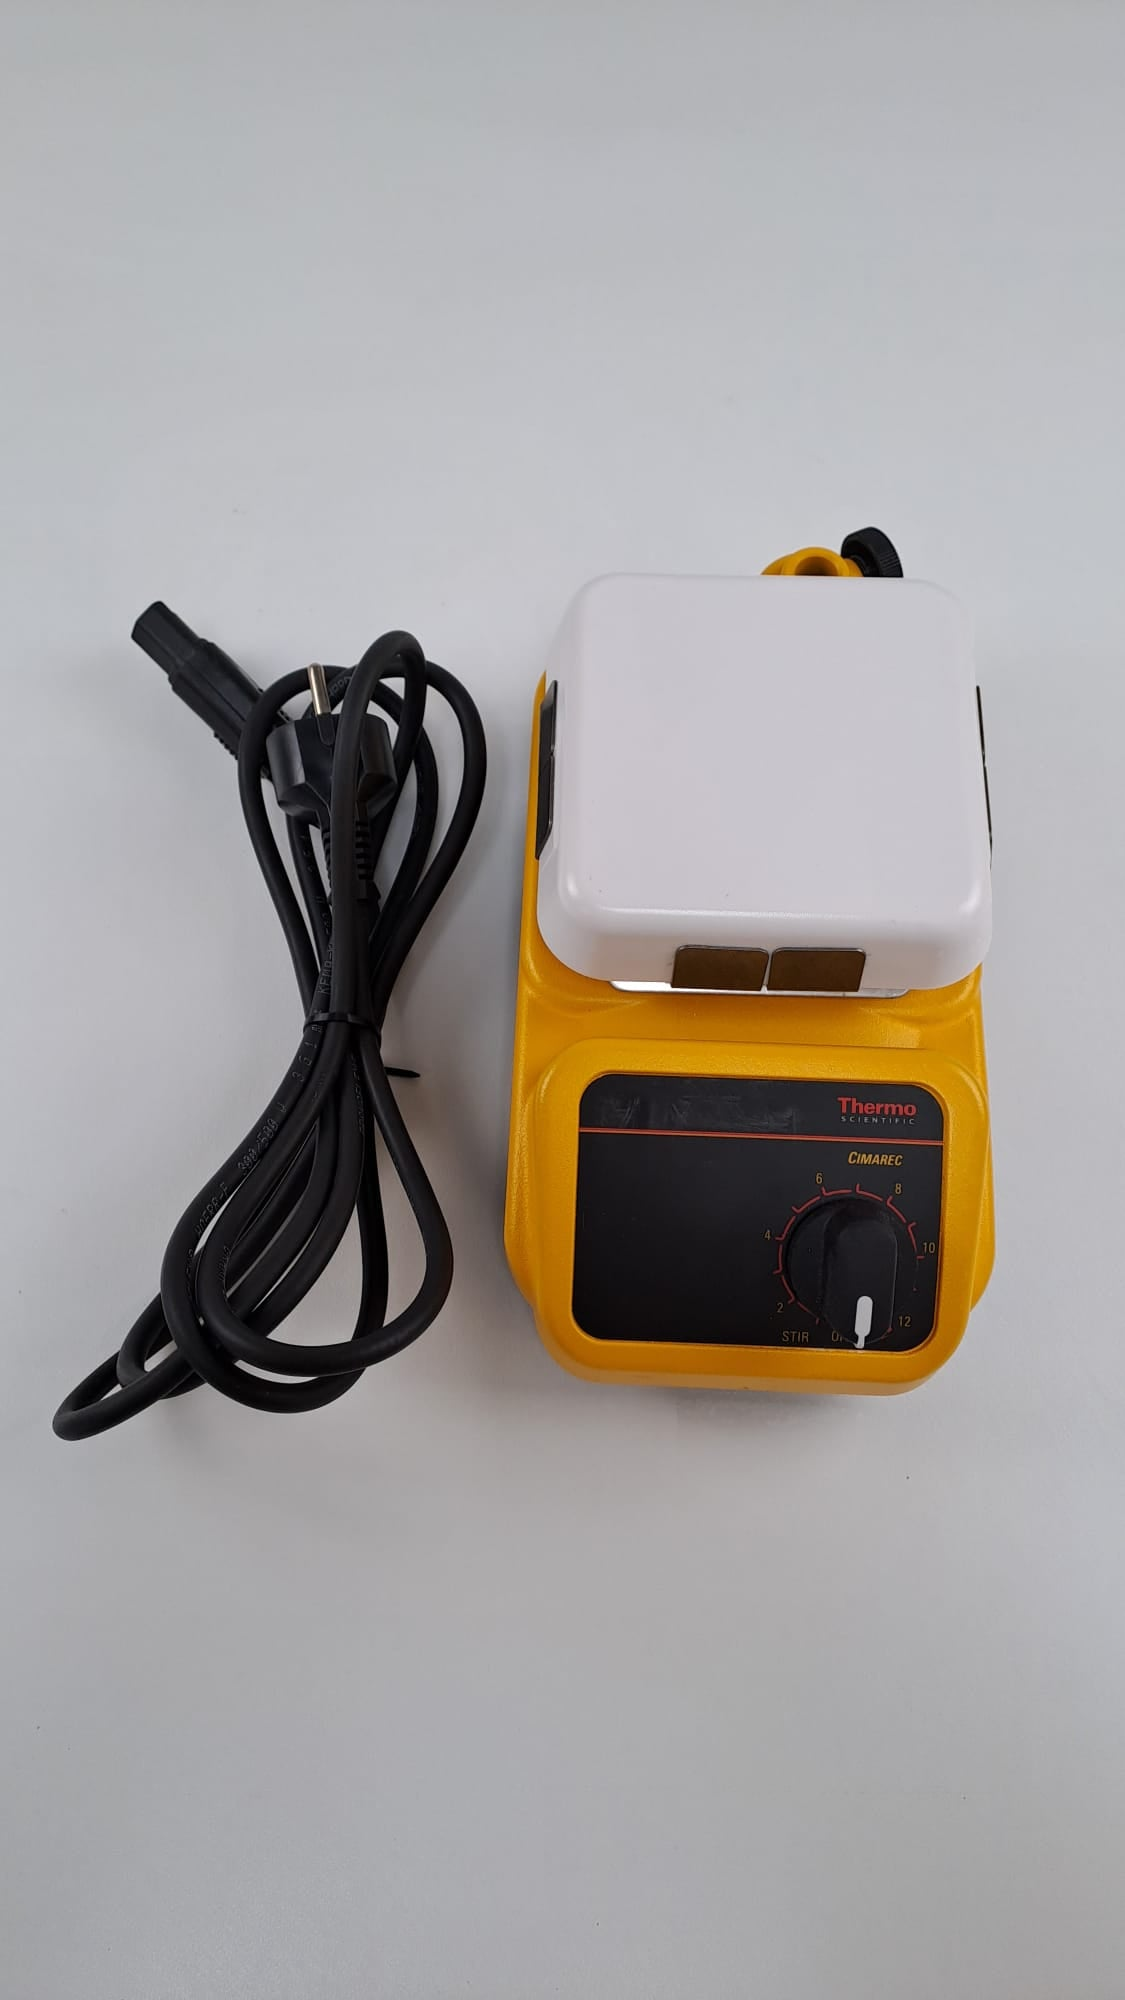
\includegraphics[width=\textwidth]{figures/agitateur3.jpg}
    \end{minipage}
    \hspace{0.2cm} % Espace horizontal entre les images
    \begin{minipage}[c]{0.45\textwidth}
        \centering
        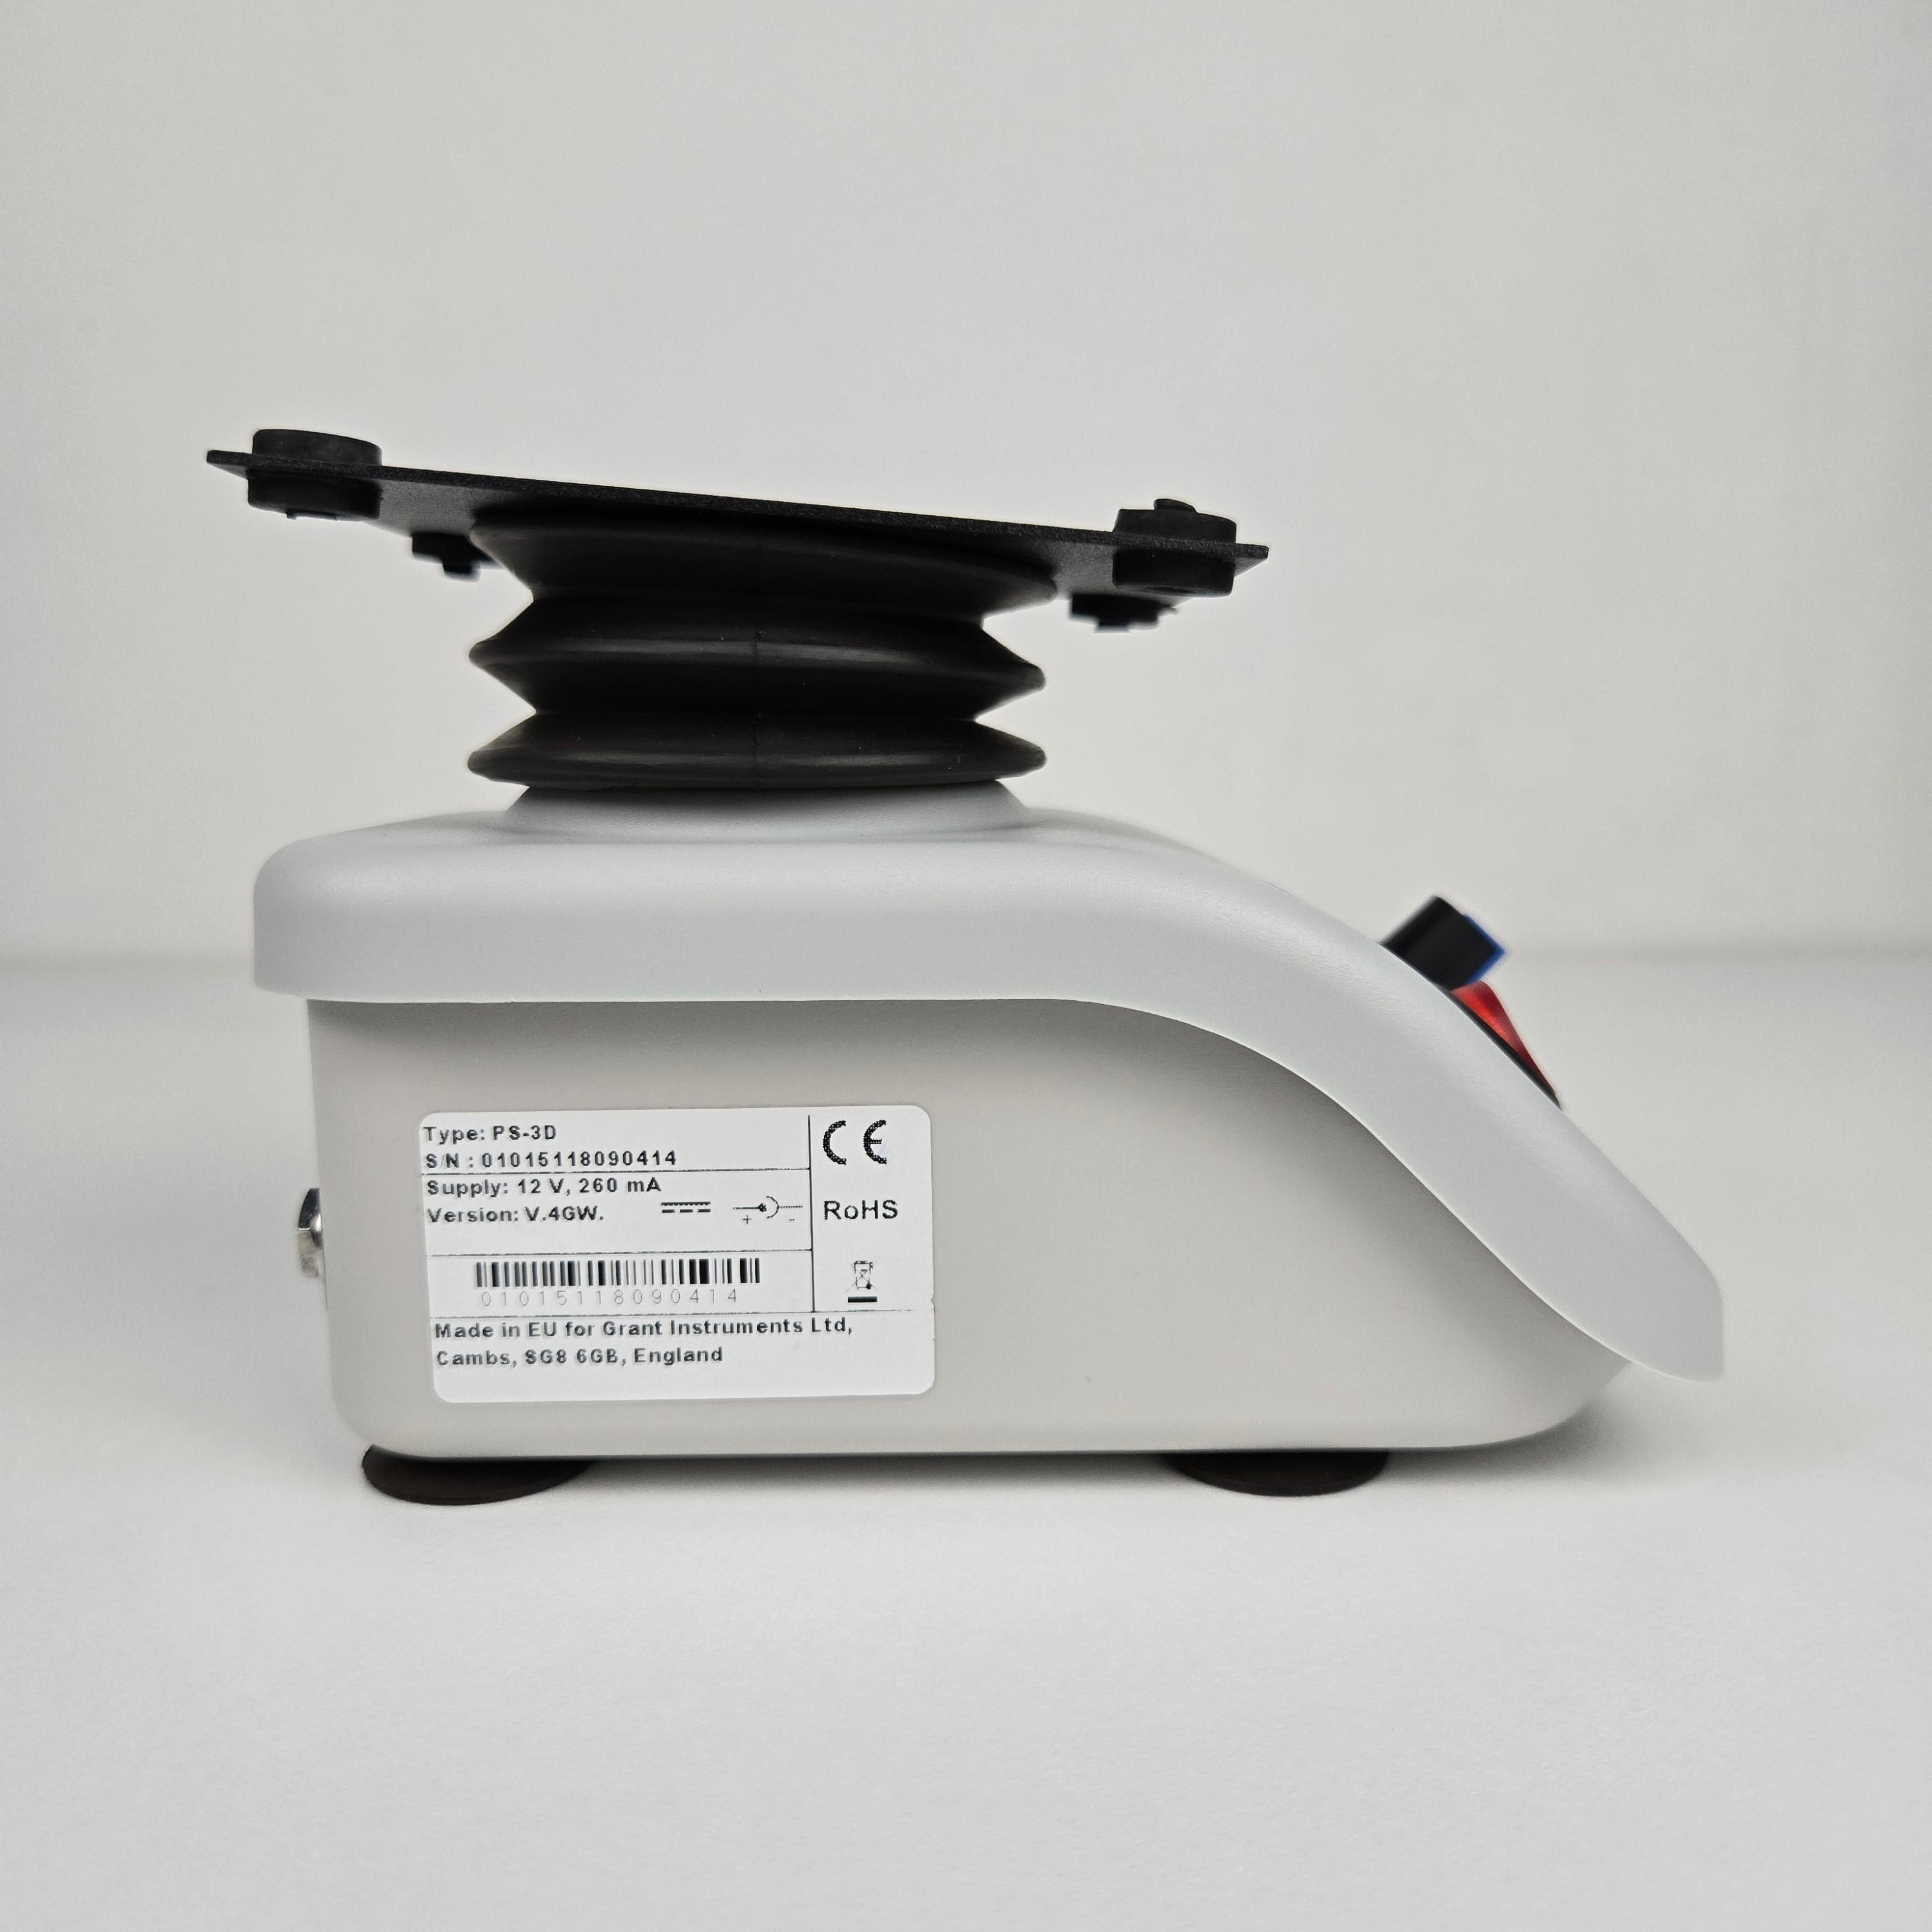
\includegraphics[width=\textwidth]{figures/agitateur4.jpg}
    \end{minipage}
    \caption{Exemple de photographies prises à destination du site web}
    \label{fig:photobrutbonus}
\end{figure}

Par exemple, sur la première image de la Figure \ref{fig:photobrutbonus}, il a été décidé d'ajouter cette photographie avec le câble d'alimentation tandis que la seconde photo a été prise pour que le client puisse se renseigner sur les caractéristiques techniques du produit figurants sur l'étiquette.

Cela se faisait au travers d’un dialogue avec mon coéquipier sur les caractéristiques du produit. Ainsi il pouvait être choisi de photographier une étiquette, un accessoire ou  autre prise de vue du produit.


\subsubsection{Inventaire du matériel de laboratoire jetable}
L’inventaire de Rewake était en cours de réalisation lors de mon arrivée en stage. L’ingénieur process nous a demandé à moi et mon coéquipier d’établir l’inventaire des produits à usage unique (pipettes, seringues stériles, bouchons d’aluminium) et de répartir les stocks sur deux palettes de sorte à que chaque produit soit facilement accessible. 

Le travail consistait à prendre un carton de produits, à en déballer un pour définir ses caractéristiques (et s’assurer de ne pas le confondre avec une autre produit), à le photographier à destination du site puis à l’inventorier en comptant le nombre de produits pour enfin le déposer sur une des deux palettes choisies.

Ce travail nécessitait un dialogue entre moi et mon coéquipier ainsi que l’ingénieur process afin de déterminer les frontières entre deux produits très semblables. Par exemple, devions nous compter des bouchons de différentes couleurs comme deux produits distincts ? Peut-on considérer des fioles de même volume et précision mais de marque différente comme un seul produit ? Il était ensuite nécessaire de préciser dans la description du produit dans l’inventaire les particularités de celui-ci par rapport aux produits semblables afin qu’aucune ligne de l’inventaire ne soit confondue avec une autre.

De la même manière il était nécessaire de bien comprendre l’utilisation future des deux palettes de stockage afin de correctement positionner les produits dessus. Il fut choisi de repartir les objets semblables dans les mêmes compartiments quitte à devoir enlever l’emballage d’origine du produit afin d’optimiser l’espace.

\subsection{Travaux dans les bureaux de l'entreprise}

Le travail demandé dans les bureaux de Montreuil ou à station F était exclusivement un travail informatique. Trois grandes tâches m'ont été demandées : l'actualisation des inventaires de Rewake, le profilage de potentiels clients et la retouche des photographies à destination commerciale.

La supervision a été réalisée en grande partie par les deux dirigeants : Alban Catoire et Paul Forget. Les tâches demandées était la plupart du temps individuelles ou réalisées en parallèle par mon coéquipier stagiaire sans nécessiter autant de coordination que ce qu'exigaient les travaux dans l'atelier.

\subsubsection{Profilage client}
\label{subsubsec:profilage}
La connaissance de l'écosystème dans laquelle évolue l'entreprise est vitale pour une startup s'inscrivant dans une démarche d'économie circulaire. En effet, Rewake a besoin à la fois de trouver des acheteurs potentiels de ses produits reconditionnés, mais également des revendeurs ou donneurs de matériels de laboratoire usagés. Également il est nécessaires pour l'entreprise de connaître les réparateurs qu'elle peut contacter dans ses démarches de réparation et ceux qui lui sont concurrents. Enfin, elle doit par sa stratégie de marque, se faire reconnaître par le milieu scientifique privé et public afin que la qualité de ses services soit reconnue.

Deux grands travaux de profilage m'ont été demandés au cours de mon stage :
\begin{itemize}
    \item Recherche de contact dans les laboratoires de travaux pratiques d'établissements privés et publics (CPGE privées, DUT, grandes écoles, etc...)
    \item Profilage de chefs d'entreprise participant à un salon auquel Rewake s'apprêtait à participer et potentiellement intéressés par les services de l'entreprise.
\end{itemize}
Ces deux tâches consistaient à remplir pour chaque entité une ligne d'un tableau tel que proposé dans la Table \ref{tab:contact_poste}.

\begin{table}[H]
\centering
\begin{tabularx}{\textwidth}{|c|c|c|c|X|}
\hline
\textbf{Nom} & \textbf{Prénom} & \textbf{Entreprise} & \textbf{Poste} & \textbf{Contact} \\ \hline
McDowall & Bob & R.D.McDowall Limited & Directeur & Email, Numéro de téléphone ou lien Linkedin \\ \hline
\end{tabularx}
\caption{Informations de contact des personnes profilées}
\label{tab:contact_poste}
\end{table}

Ce travail nécessitait de savoir faire des recherches avancées via un moteur de recherche afin d'être efficace dans la recherche d'information de la personne cible. Par exemple l'usage du mots-clés \texttt{site:} permettant de chercher les mots clés de la recherche exclusivement sur un site web (Linkedin ou le site d'un l'institut par exemple) d'accélére grandement les recherches. De même l'utilisation des guillemets \texttt{""} ou du point d'exclamation \texttt{!} imposant respectivement  l'apparition d'un mot-clef ou l'excluant de la recherche web, d'exclure les pages liées à un homonyme.

La principale difficulté de ce travail résidait, comme tout travail de recherche, dans la décision de savoir quand nos efforts devaient s'arrêter vis-à-vis des vérités que l'on cherchait à établir. Ainsi, il fut souvent question de savoir s'il valait la peine de continuer de chercher de potentiels liens de contact d'une personne dont on n'avait réussi à collecter qu'un compte Linkedin peu actif ou plutôt de passer à une personne suivante. 

Ces questionnements ont été d'abord résolus par les deux dirigeants qui m'ont indiqué quelles étaient les personnes prioritaires de ma liste pour lesquelles il valait la peine de s'attarder. Puis, par habitude de la tâche, il est devenu aisé, après une trentaine de profils déjà remplis de "deviner" en fonction des résultats de recherche si les informations à acquérir sur la personne seraient faciles à obtenir ou très longues, et si des travaux d'investigation plus longs amèneraient a des résultats ou non.


\subsubsection{Détourage des photographies commerciales}
\label{subsubsec:photoshop}
La plupart des photographies destinées à la vente des produits sur le site Web de Rewake sont prises depuis l'entrepôt de Montreuil dans un espace studio photo dédié. Cependant, afin de conserver la cohérence esthétique du site, il est nécessaire de remplacer l'arrière-plan des produits par un fond blanc plus épuré. Ceci a été réalisé grâce au logiciel de retouche \texttt{Adobe Photoshop}. Cette tâche qui m'a été proposée par les deux dirigeants a été réalisée en autonomie.

\begin{figure}[H]
    \centering
    \begin{minipage}[c]{0.45\textwidth}
        \centering
        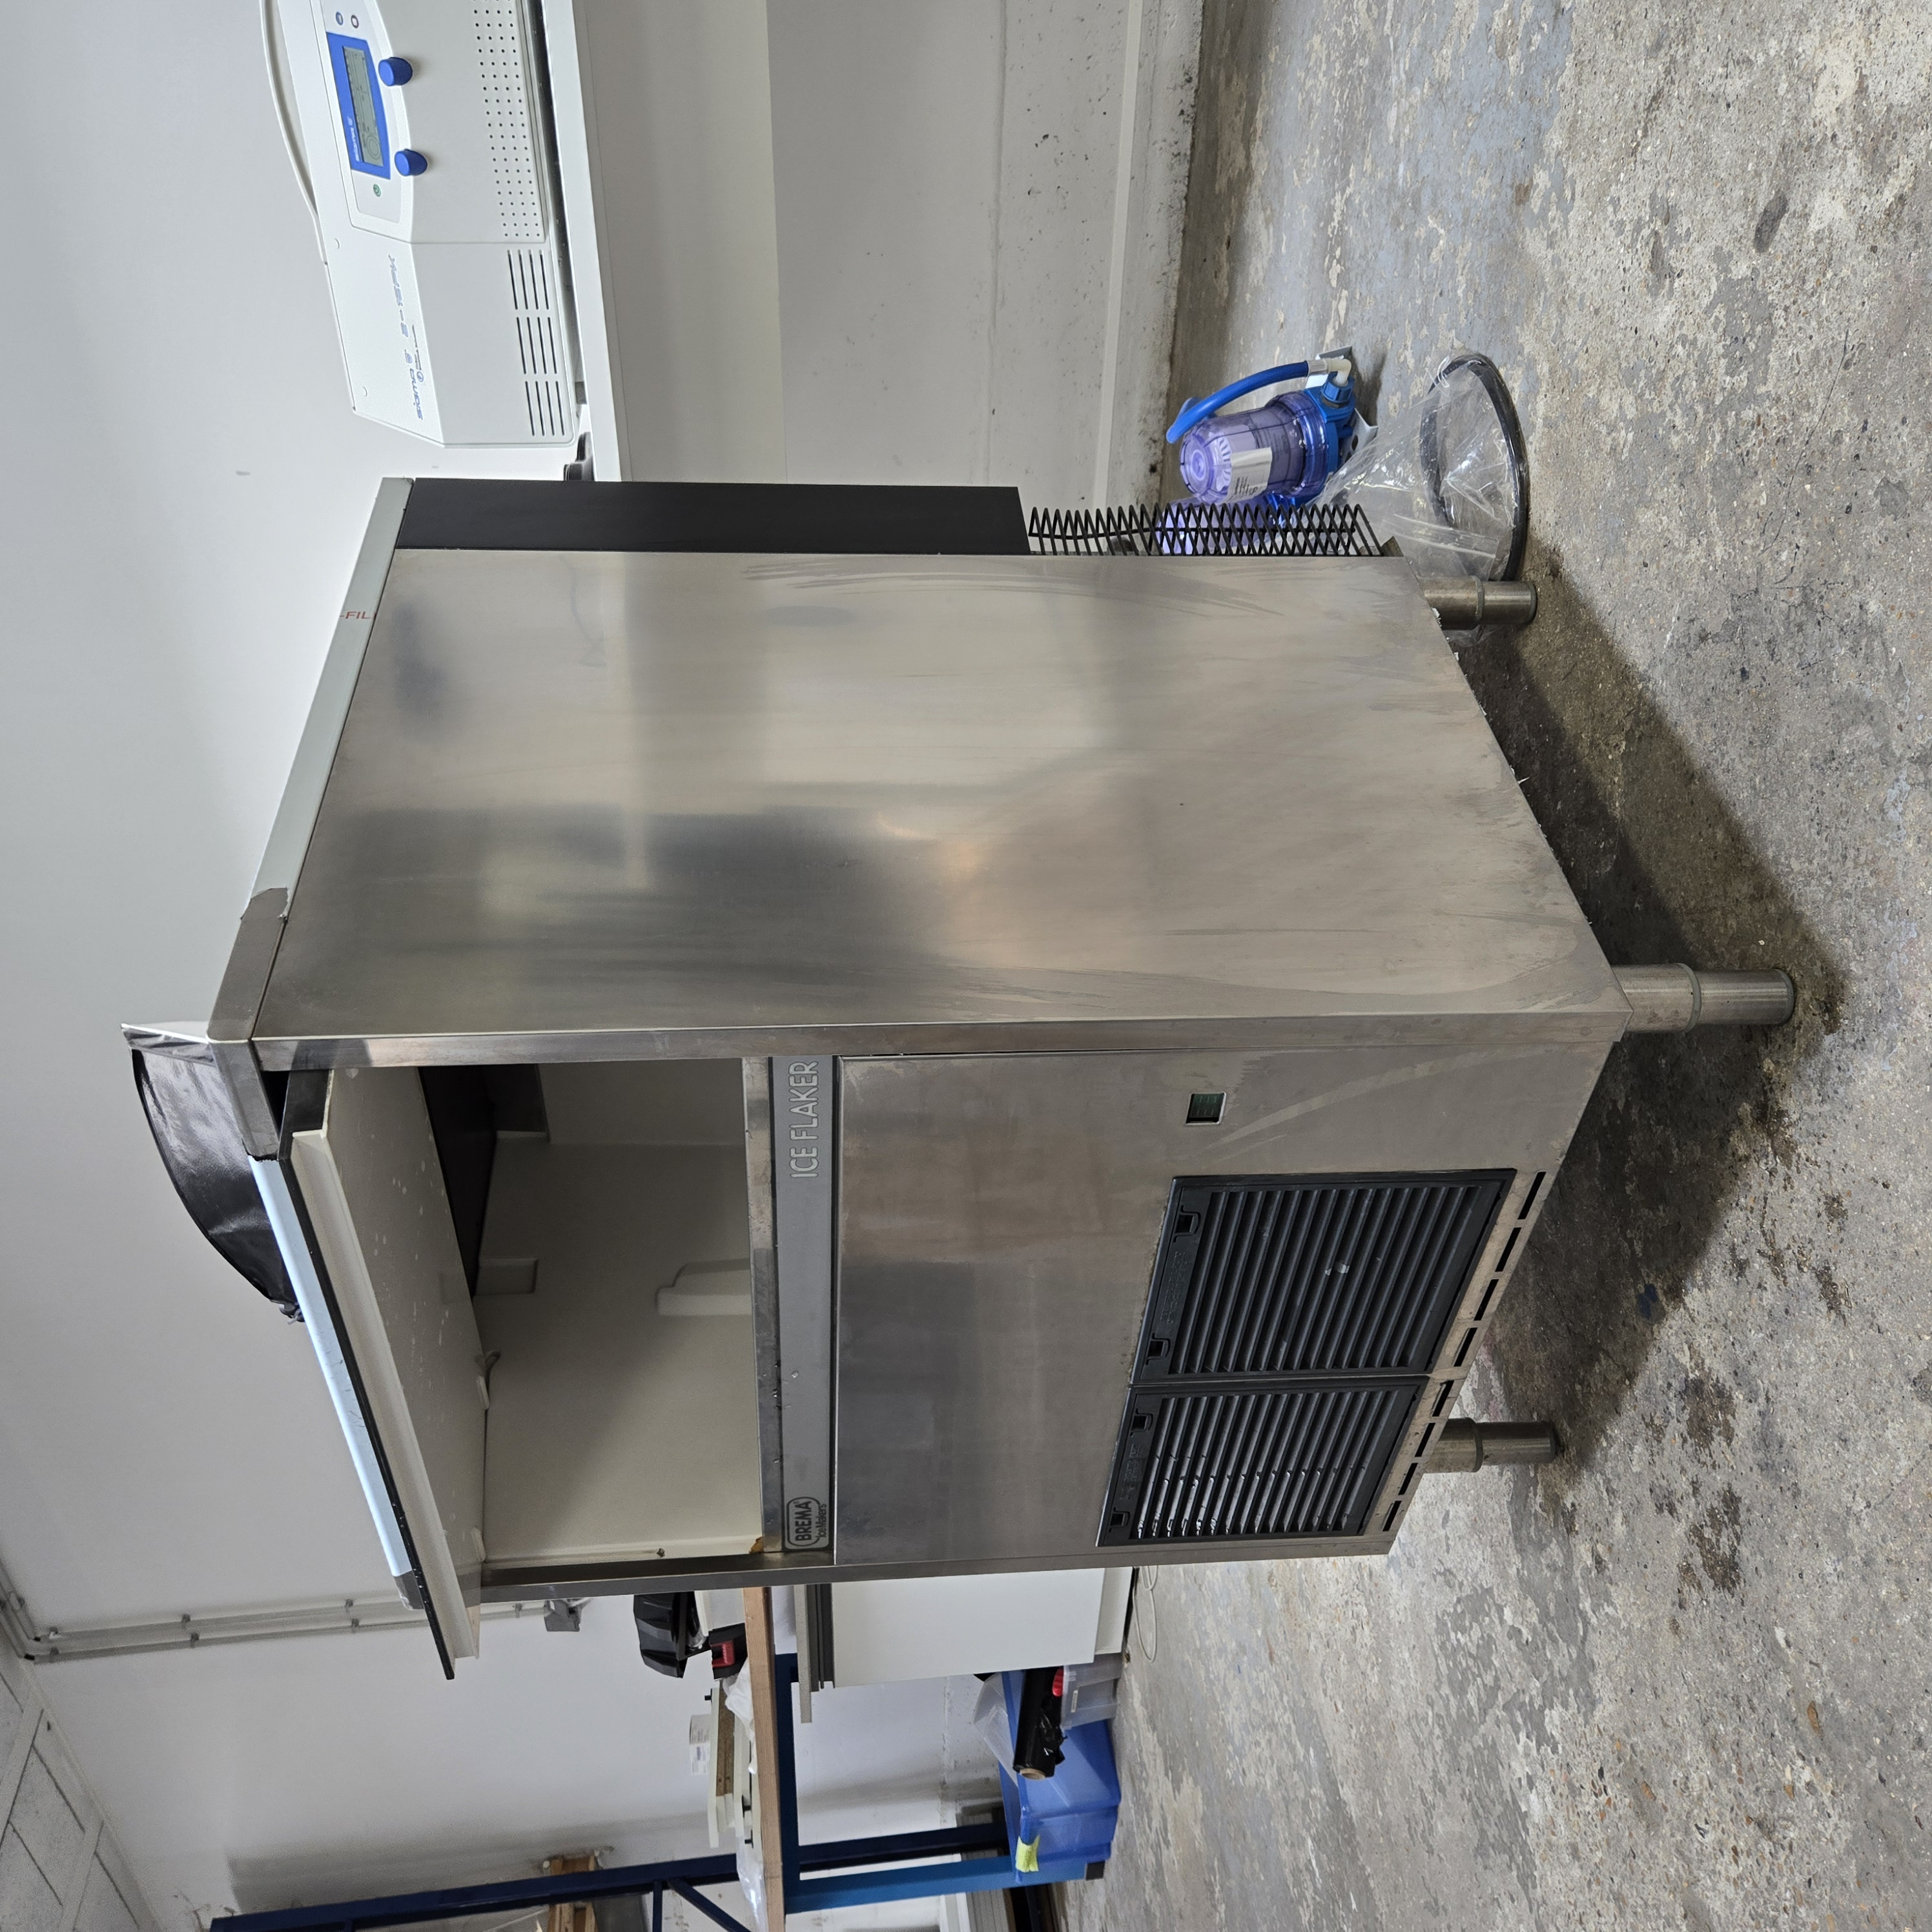
\includegraphics[width=\textwidth, angle=270]{figures/machinglace.jpg}
    \end{minipage}
    \hspace{0.2cm} % Espace horizontal entre les images
    \begin{minipage}[c]{0.45\textwidth}
        \centering
        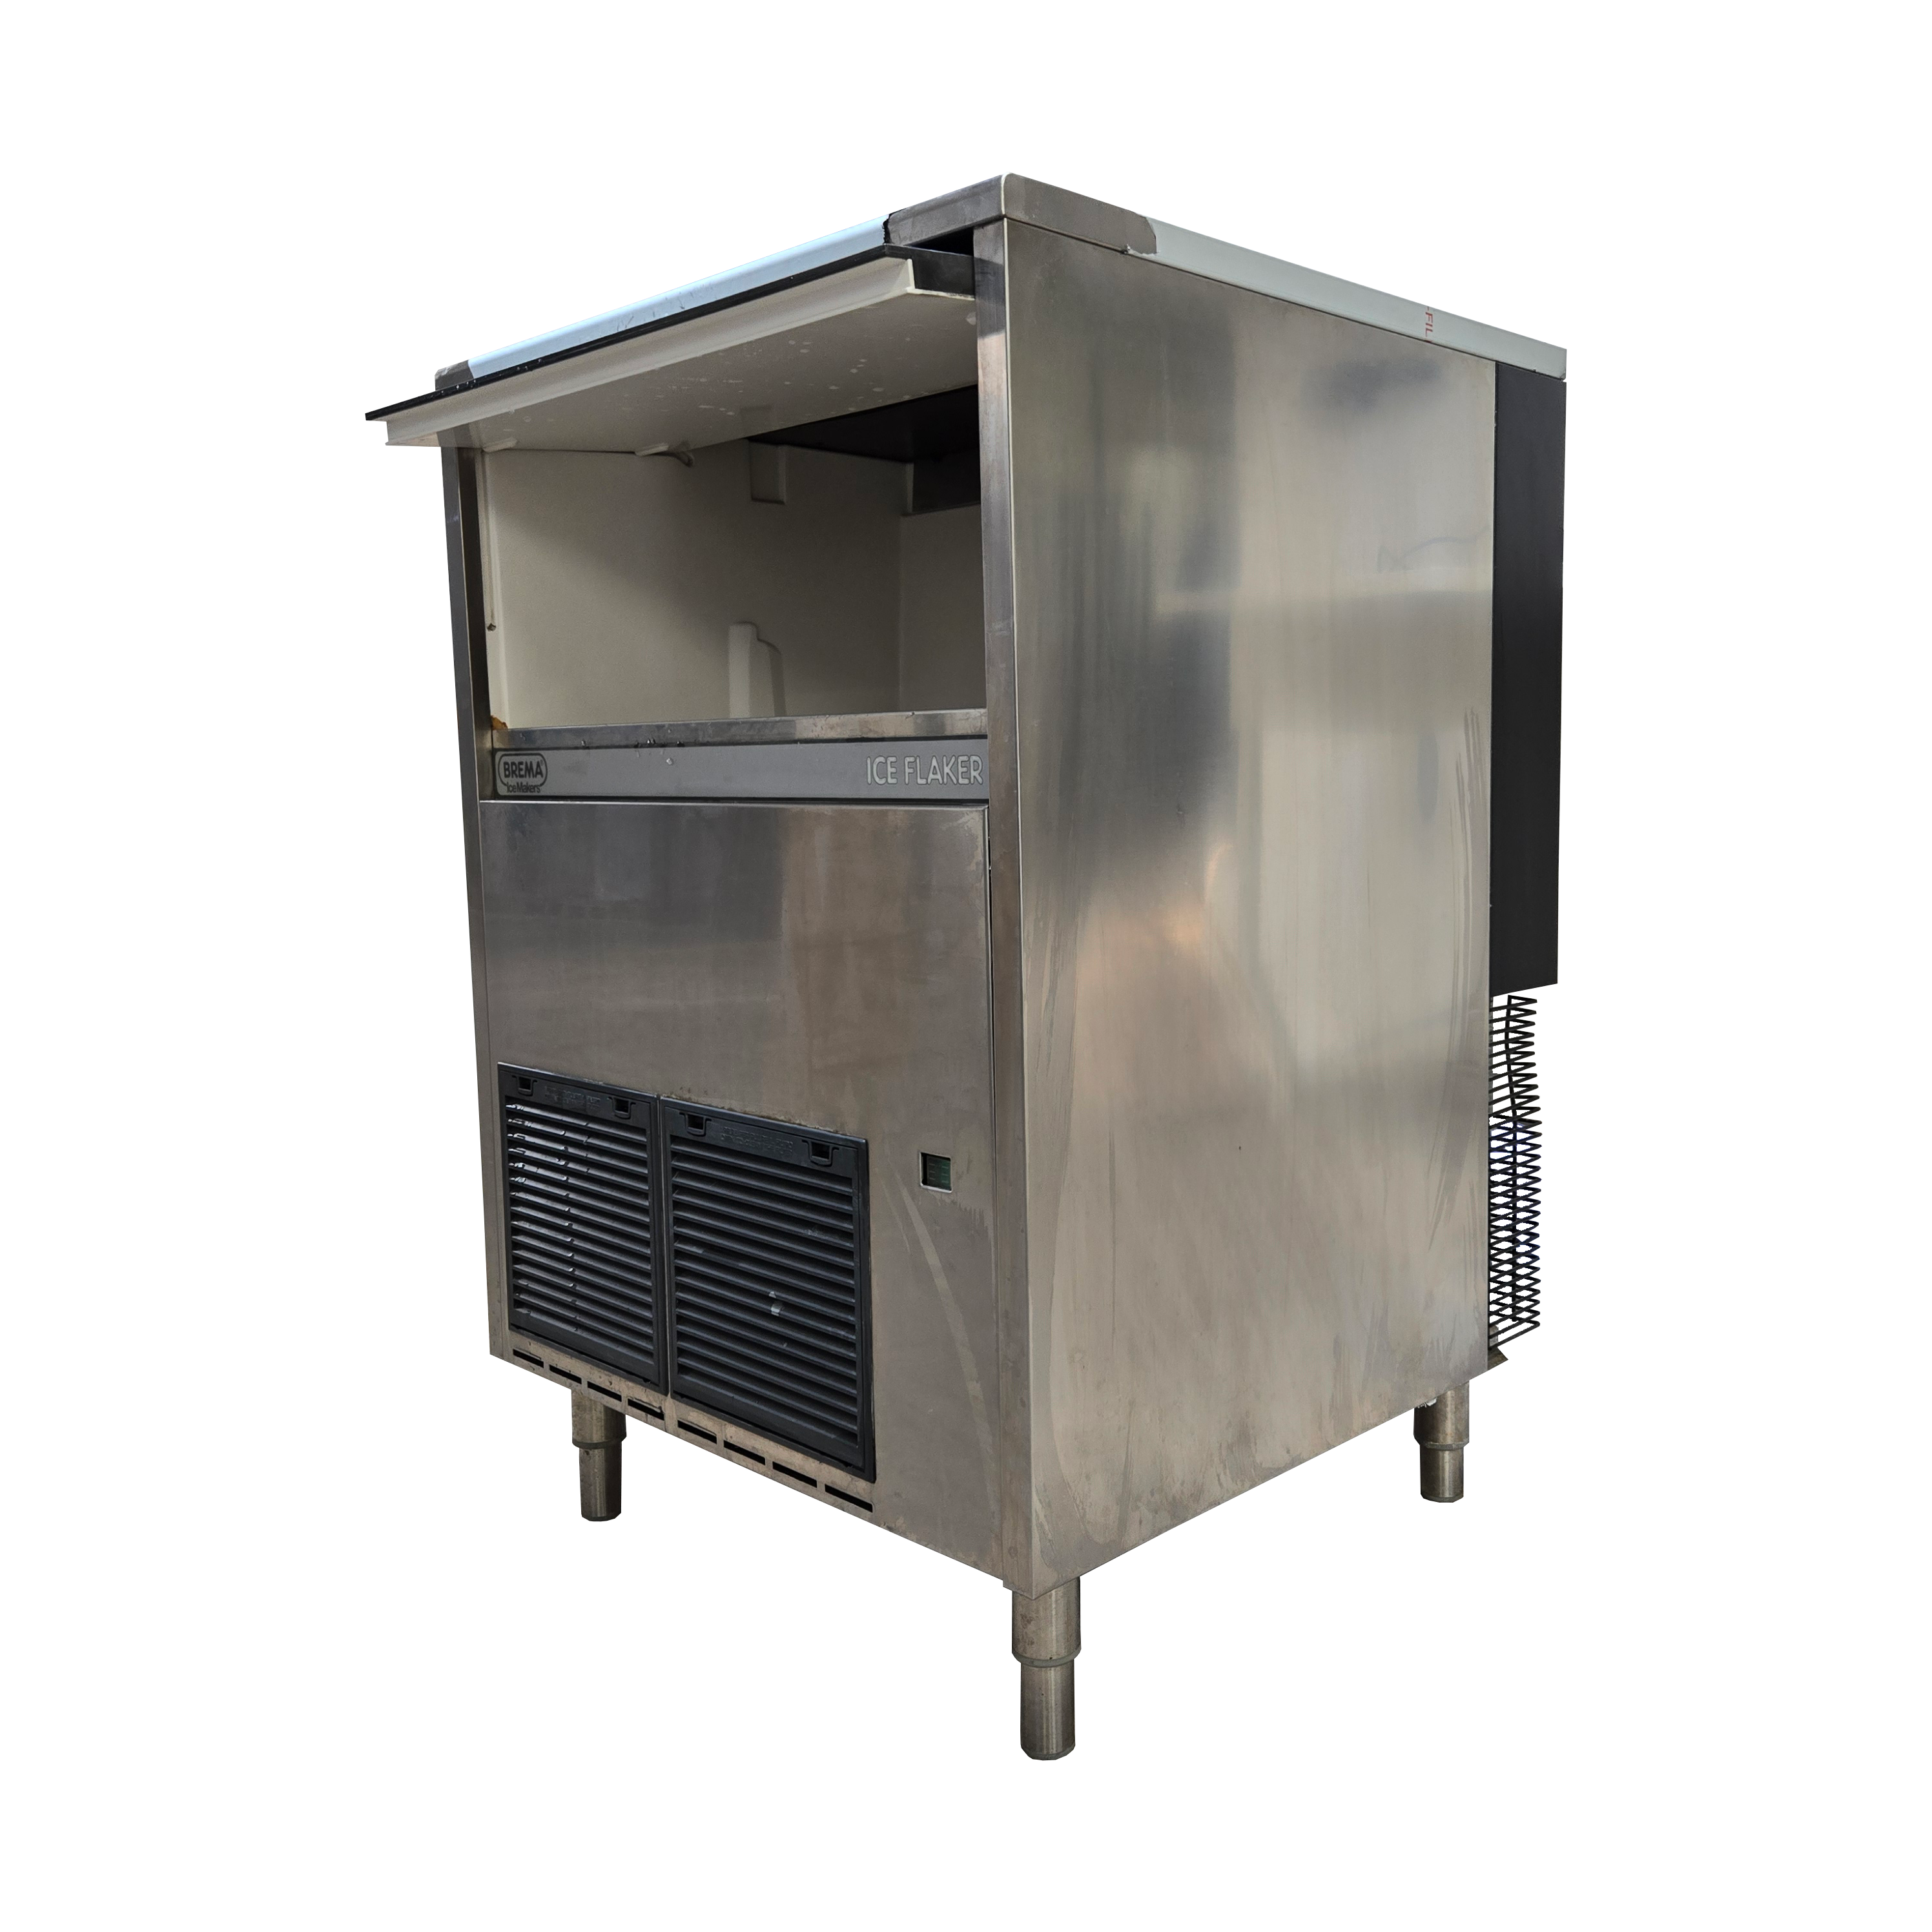
\includegraphics[width=\textwidth]{figures/machinglace.png}
    \end{minipage}
    \caption{Exemple avant/après d'une retouche photo}
    \label{fig:avantapres}
\end{figure}

Cette tâche nécessitait une connaissance préalable avancée du maniement du logiciel \texttt{Adobe Photoshop}, des différents outils de séléction qu'il propose et de de leur emploi, permettant leur utilisation à bon escient afin de réaliser ce travail esthétique le plus rapidement possible.

Les objectifs de cette tâche ont été à plusieurs reprise reconsidérées entre le CEO et moi-même. En effet, il a été initialement prévu que je détoure l'ensemble des photos présentes sur le site web. Cependant, face à l'avancement tardif vis-à-vis des attentes de mon dirigeant, il a donc été décidé finalement que je ne détourerais uniquement la photographie principale de chaque produit. 

\begin{figure}[H]
    \centering
    \begin{minipage}[c]{0.45\textwidth}
        \centering
        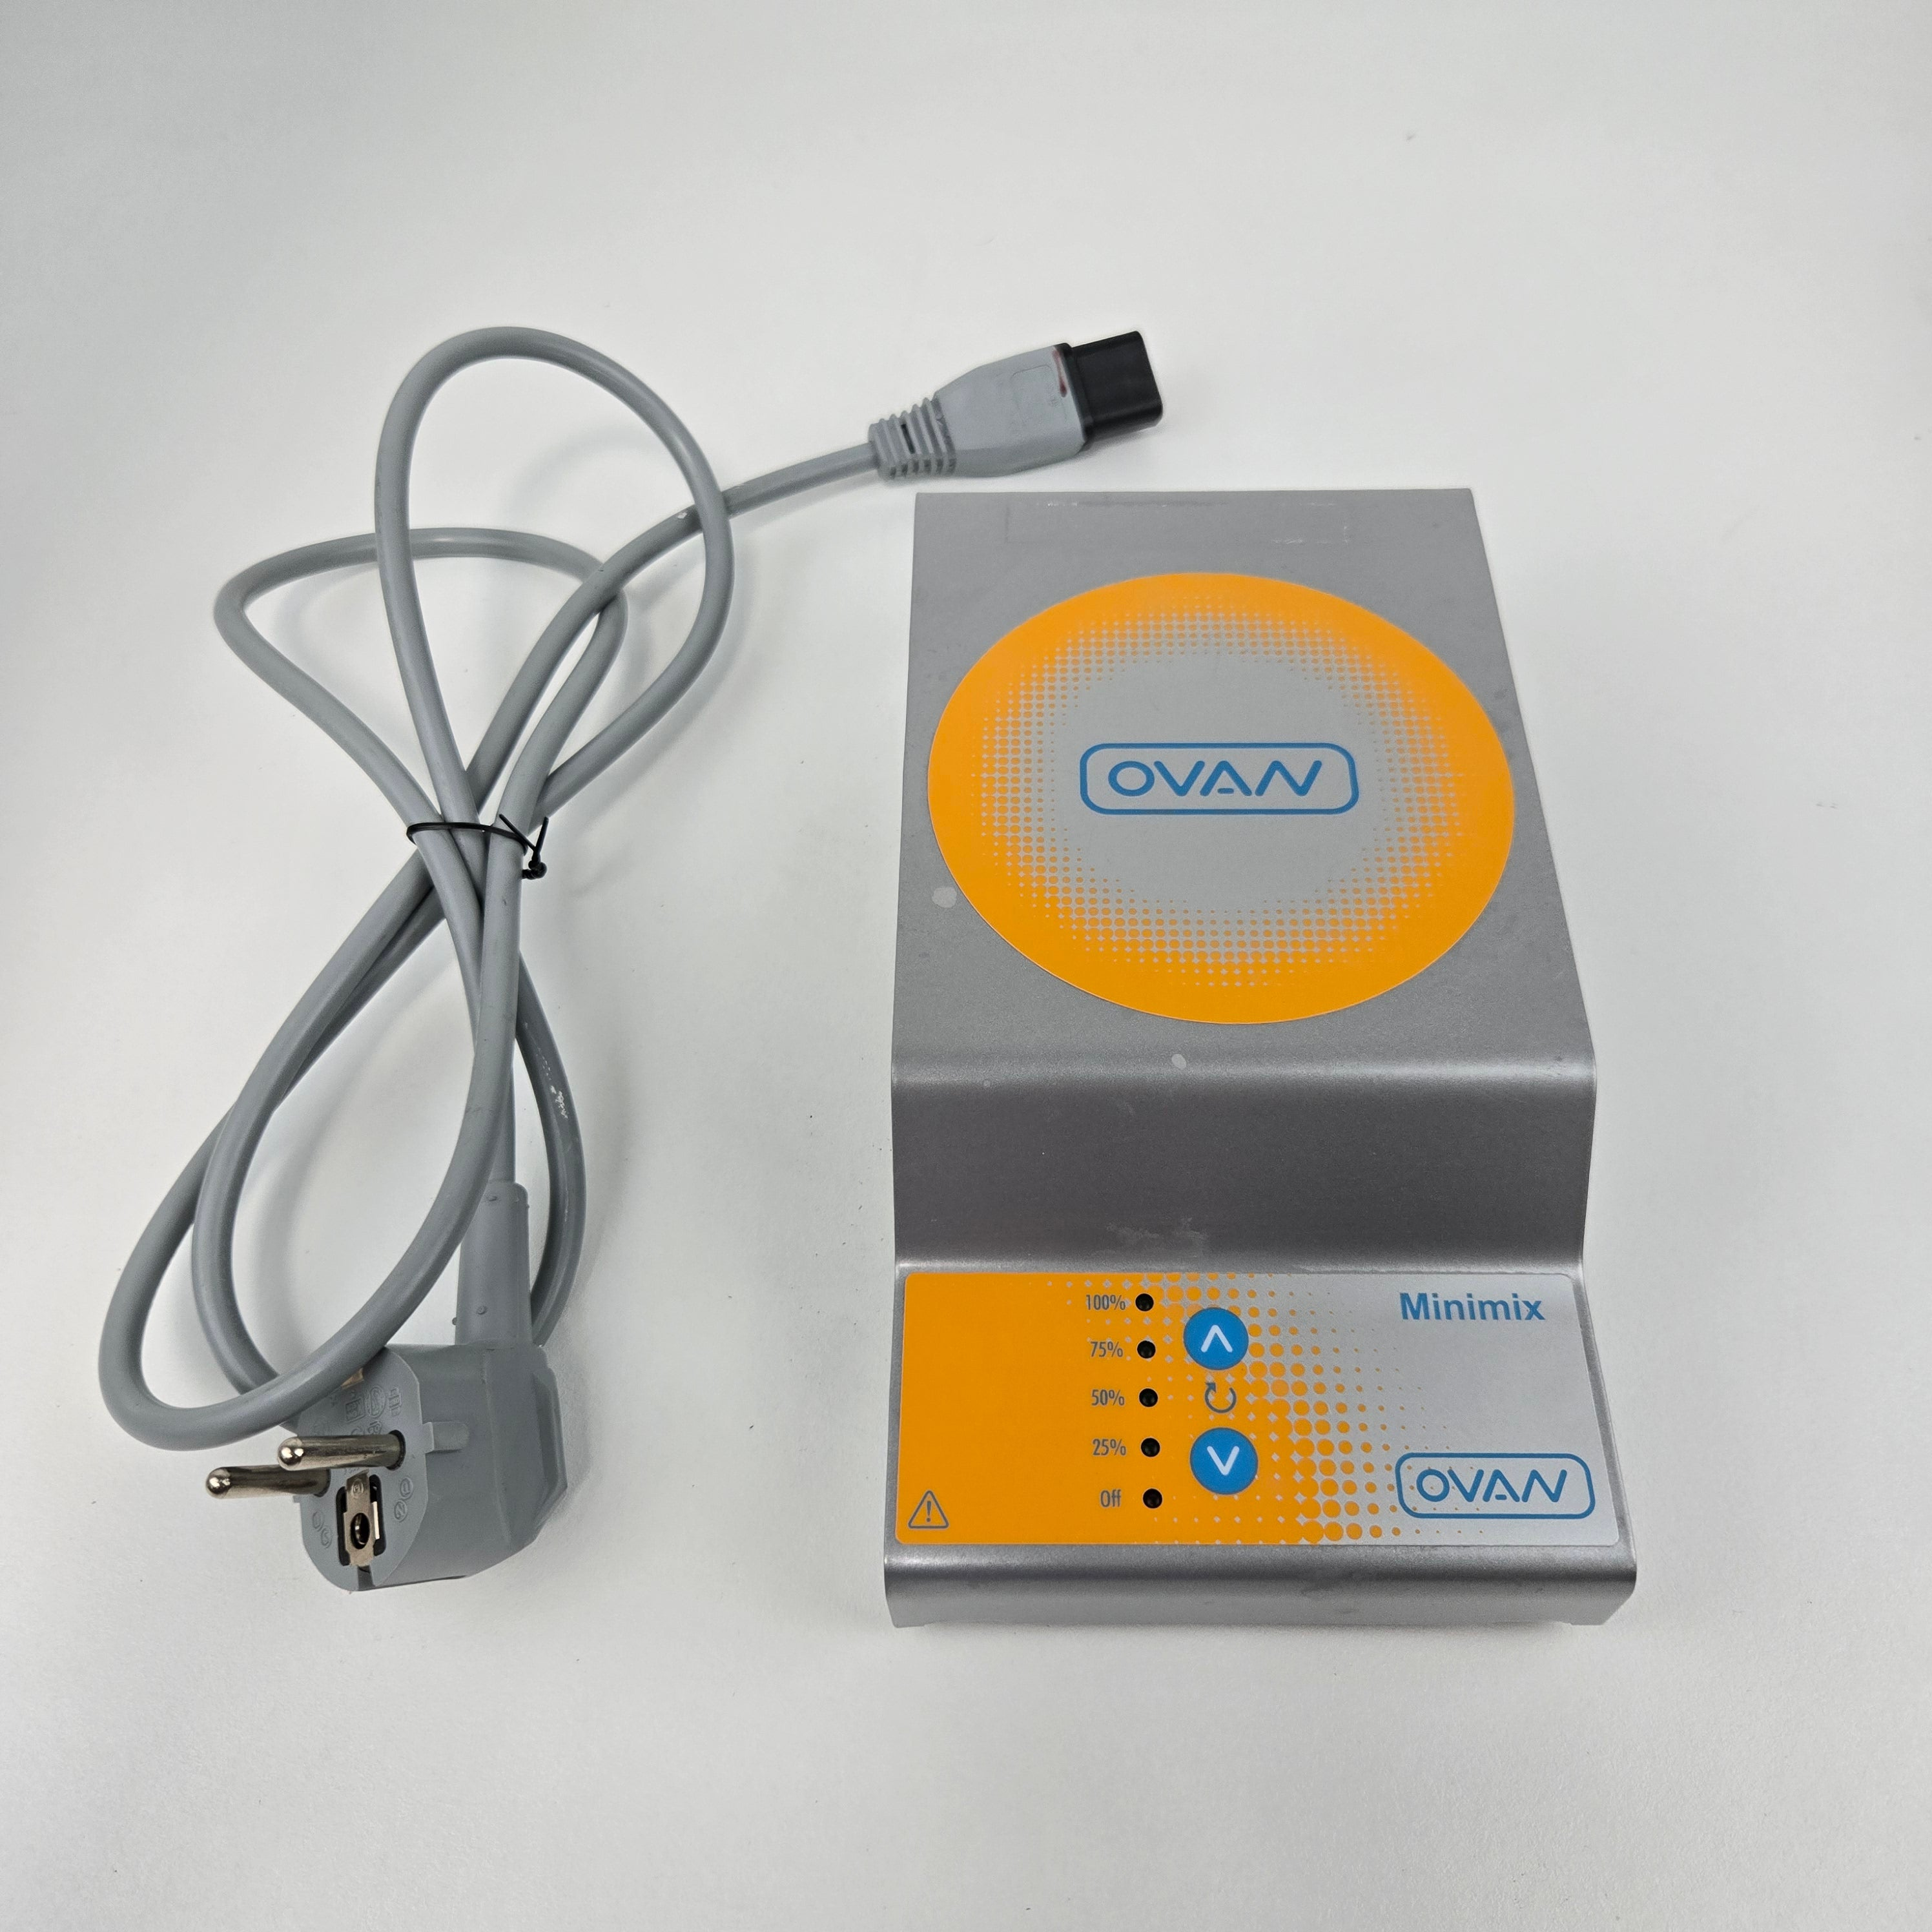
\includegraphics[width=\textwidth, angle=0]{figures/agitateur5.jpg}
    \end{minipage}
    \hspace{0.2cm} % Espace horizontal entre les images
    \begin{minipage}[c]{0.45\textwidth}
        \centering
        
\includegraphics[width=\textwidth]{figures/agitateur5.png}
    \end{minipage}
    \caption{Exemple avant/après d'une retouche photo ayant demandé trop de temps de réalisation}
    \label{fig:avantapres2}
\end{figure}

Quelques temps après, il fut également décidé que certains accessoires des produits pouvaient être simplement rognés plutôt que détourés me faisant gagner un temps conséquent. La Figure \ref{fig:avantapres2} illustre un montage trop coûteux en temps : le décourage de l'alimentation électrique ayant pris trois quarts du temps de la retouche photo sans pour autant apporter un réel intérêt pour le client.

\subsubsection{Gestion des stocks et cohérence des différents inventaires}

À mon arrivée dans l'entreprise, Rewake disposait de deux inventaires distincs et encore incomplets : 
\begin{itemize}
    \item Un inventaire des produits appartenant à Rewake dans un document \texttt{AirTable}.
    \item Un inventaire des produits mis en ligne sur le site web via la plateforme \texttt{Shopify}.
\end{itemize}

L'objectif fixé par le CEO était de fusionner ces deux inventaires en un seul disponible sur \texttt{Airtable}. Ma tâche consistait alors à faire correspondre les lignes de l'inventaire \texttt{Shopify} avec celles des tables \texttt{Airtable} puis d'ajouter les colonnes uniquement présentes sur les tables de \texttt{Shopify} (description du produit, caractéristiques techniques, prix) dans celles des tables \texttt{Airtable}.

\begin{figure}[H]
    \centering
    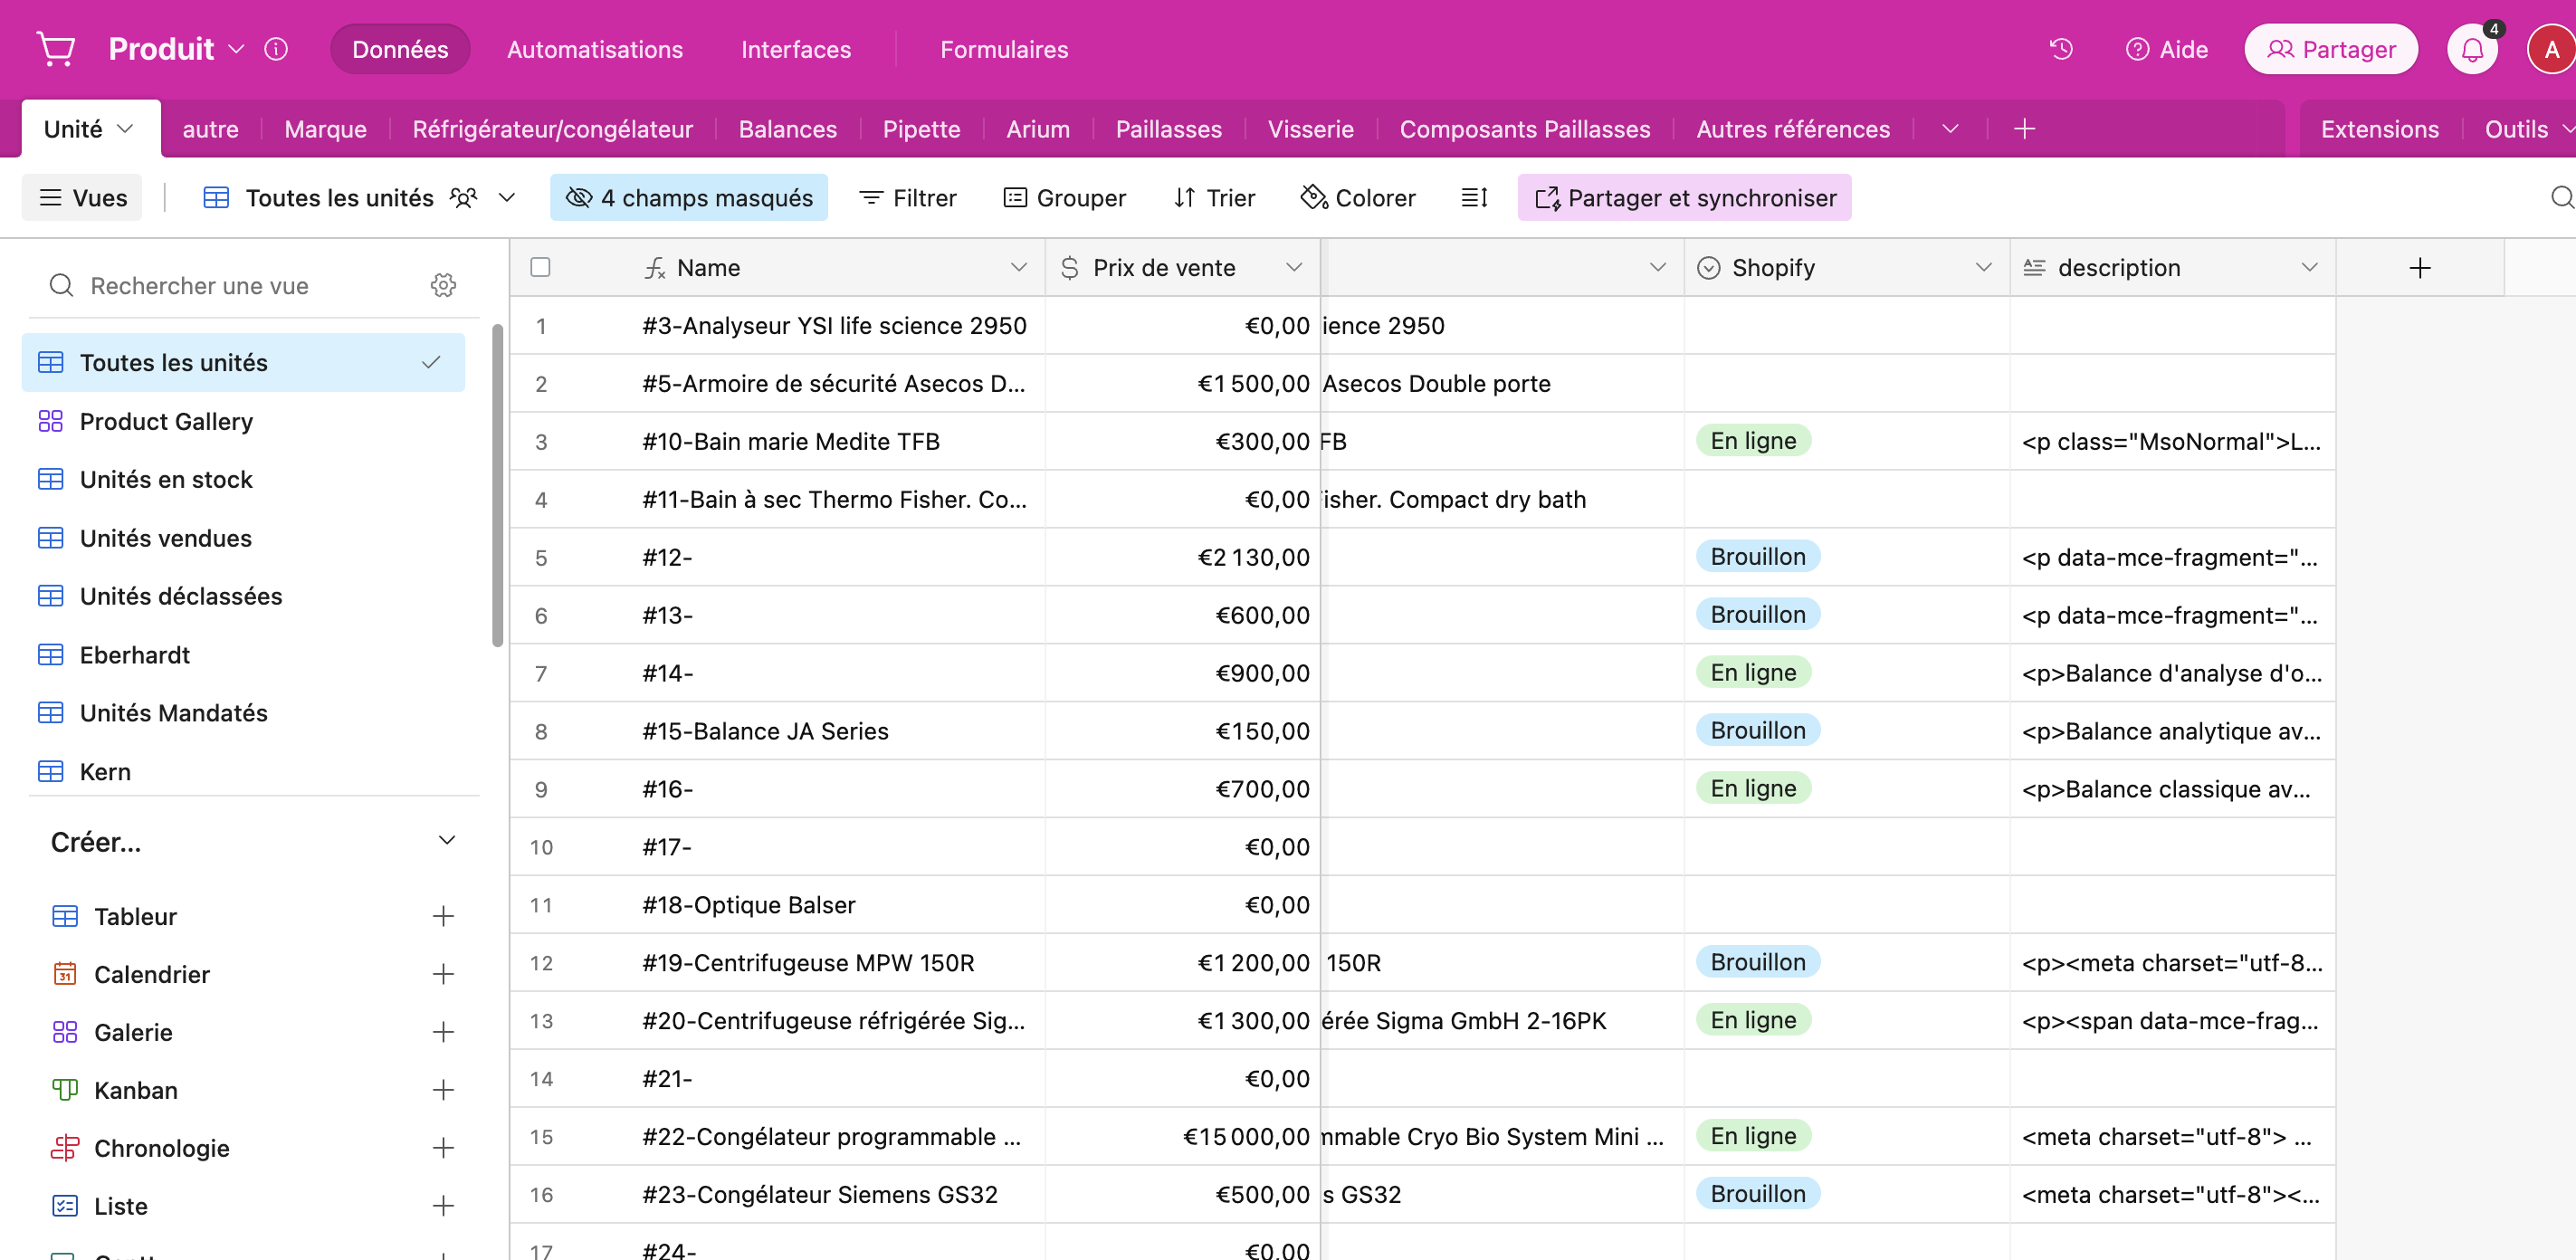
\includegraphics[width = 1\textwidth]{figures/airtable.png}
    \caption{Extrait de la table \texttt{Airtable} des réfrigérateurs}
    \label{fig:airtable}
\end{figure}

Cette tâche bien que répétitive a été réalisée sans grande difficulté, une bonne approche des deux logiciels de traitements de données permettant d'efficacement collecter les informations demandées et de les retranscrire au bon endroit.

\section{Organisation du travail}
\subsection{Mode de coordination}
Lors de mon stage, j'ai essentiellement dû coordonner mon travail avec mes collaborateurs par ajustement mutuel et plus rarement par supervision directe. Ceci est une conséquence de la structure simple de la startup Rewake, qui ne possède pas encore de protocole standardisé des tâches à réaliser lors du reconditionnement de ses produits. 
\subsubsection{Exemple d'ajustement mutuel}
La réalisation des retouches photos tels que décrites dans le chapitre \ref{subsubsec:photoshop} a été une bonne expérience d'ajustement mutuel. En effet, cette tâche étant nouvelle tant pour le CEO que pour moi-même, aucun de nous ne connaissait exactement le temps à sa réalisation. Finalement, il fut admis d'un commun accord qu'il était nécessaire de réviser la quantité de photos à retoucher. Puis venant d'une demande de ma part, qu'il était légitime que je rogne certains accessoires des produits trop complexes à détourer en un temps raisonnable.

Un autre exemple d'ajustement mutuel lors de ce stage fut le nettoyage des paillasses tels que décrit au chapitre \ref{subsubsec:paillasse}. En effet, mon coéquipier et moi-même s'occupant de nettoyer la même paillasse en même temps, il fut nécessaire d'adapter nos gestes mutuellement. Par exemple, il était nécessaire d'attendre que l'évier soit entièrement nettoyé avant de laver les planches intérieures de la paillasses. Cela demandait donc de prévoir le temps que prendrait le coéquipier à cette tâche et de trouver d'autres activités de nettoyage à réaliser pendant ce temps sur la paillasse pour l'embellir. Ce n'est qu'après plusieurs nettoyages de paillasses qu'une véritable coordination efficace a pu prendre place, laissant peu de place aux temps morts et accélérant grandement la cadence des travaux.

\subsubsection{Supervision directe}
La réparation de l'agitateur multiposte, décrit au chapitre \ref{subsubsec:multiposte}  est un bon exemple de supervision directe. En effet, j'ai pendant cette activité exécuté immédiatement les instructions que me donnait l'ingénieur process afin de remplacer la courroie. Il commentait en direct mes gestes afin que je les affine selon son expérience permettant un bon déroulé du procédé qu'il avait imaginé.

Un autre exemple de supervision directe quoique plus souple fut le profilage des clients tel que décrit dans le chapitre \ref{subsubsec:profilage}. En effet, mon superviseur passait régulièrement vérifier que la tâche avançait selon son exigence de rapidité et que j'avais obtenu les bons contacts pour les personnes déjà repérées.

\subsection{Type de tâches}
La variété des tâches exécutées durant ce stage fait bien évidemment penser que le mode d'organisation des tâches pour le poste de stagiaire ouvrier fonctionne par \textbf{rotation des postes}. On mise ainsi sur la polyvalence des compétences de celui-ci et sa capacité à résoudre certaines problématiques de la jeune entreprise.

\section{GRH et management}
Dès les premières interactions avec mon tuteur lors de mon recrutement, j'ai pu ressentir l'environnement social dynamique et la forte identité d'entreprise propre aux jeunes startup.

\subsection{Relations sociales}
Le tutoiement a très vite était établi, dès mon premier entretien avec mon recruteur. La ligne hiérarchique ne se fait vraiment ressentir que lorsque les consignes de travail pour la journée sont établies. Le reste du temps rien dans les dialogues ne permettait de distinguer les employés des dirigeants. Cet esprit d'équipe est d'autant plus animé par les pauses du midi. En effet, les dirigeants faisant en sorte que celles-ci soient les plus conviviales possibles, nous étions invités à prendre notre déjeuner ensemble sur une des terrasses des lieux de l'entreprise, permettant de renforcer les liens entre les collaborateurs. De même, il était possible de participer à des matchs de foot avec d'autres employés d'entreprise occupant les lieux.

Sans posséder de Comité Social Entreprise, les deux dirigeants, rendent compte du bien-être des employés sur leur lieu de travail. Cela s'est illustré pour moi et l'autre stagiaire ouvrier par un entretien de mi-stage permettant un retour au CEO de l'intégration, de notre ressenti dans l'entreprise et de notre avis sur l'activité de l'entreprise et ses travaux.

\subsection{Recrutement du personnel}
Le recrutement chez Rewake se fait par entretien vidéo ou en présentiel. Lors de celui-ci l'engagement de la personne dans les domaines d'activité de l'entreprise semble avoir une grande importance. En effet, l'entreprise s'inscrit dans une démarche de développement durable et reprend dans ses prévisions de croissance les notions de "monde fini" des économistes écologistes. Il est donc important pour Rewake que son équipe entretienne les mêmes valeurs.

\subsection{Mode d'évaluation et rémunération du personnel}
Rewake n'en est encore qu'à ses premiers recrutements et n'a, à ce jour, signé aucun contrat en CDD ou CDI. Elle vise cependant à recruter un premier alternant d'ici septembre. Il est stipulé dans le pacte d'actionnaires, signé lors des levées de fonds de la startup, qu'une part des actions de l'entreprise sera attribuée aux employés en fonction de leur ancienneté.

Cette clause a été mise en place dans le but de motiver et fidéliser les employés en leur offrant une participation directe dans le succès de l'entreprise. En alignant les intérêts des collaborateurs avec ceux des actionnaires, Rewake espère encourager un engagement à long terme et une implication plus profonde dans la croissance de la startup. De plus, cette répartition d'actions vise à attirer des talents clés, en proposant une incitation financière supplémentaire au-delà des simples salaires, ce qui est souvent crucial pour une jeune entreprise en phase de développement.

\section{Responsabilité sociale et sociétale de Rewake}
La démarche de responsabilité sociétale des entreprises (RSE) de Rewake s'inscrit dans un modèle d'économie circulaire, axé sur le réemploi d'équipements de recherche et de laboratoire. L'objectif principal de Rewake est de lutter contre le gaspillage d'équipements scientifiques encore fonctionnels, qui sont souvent jetés alors qu'ils pourraient être reconditionnés et réutilisés par d'autres laboratoires. En reprenant ces équipements inutilisés, en les reconditionnant dans leurs ateliers en France et en les revendant à prix réduit, Rewake favorise une approche durable et économique. Cela permet non seulement de réduire les déchets électroniques, mais aussi d'offrir une solution abordable à des laboratoires ou projets ayant des contraintes budgétaires.

Ce modèle participe à la réduction de l'empreinte environnementale dans le secteur scientifique et s'aligne avec les principes de durabilité et de responsabilité sociale, tout en répondant aux besoins croissants en équipements de recherche de qualité à moindre coût. Rewake espère ainsi jouer un rôle actif dans la transition vers une économie plus verte et plus circulaire

Cependant, les activités de Rewake restent limités par des contraintes économiques. Par exemple, la plupart des pièces commandées pour la réparation des instruments sont exclusivement sélectionnées selon le prix sans prendre en compte la distance de transport du produit. De même, Rewake ne peut pas encore, dans son entrepôt actuel trier efficacement ses déchets ne disposant pas de toutes les poubelles adéquates. Ce sont des exemples de problématiques connues de l'entreprise qui vise à les corriger d'ici l'année prochaine montrant son implication dans sa démarche écologique.

\section{Hygiène et sécurité}
Les travaux dont l'entrepôt sont prompts à des risques physiques et chimiques. D'abord, les employés doivent déplacer de lourdes charges manuellement, à l'aide d'un transpalette ou de leur bras facteur de risque de blessure. De même le démontage de matériel usagé pouvant contenir des pièces lourdes, coupantes ou en tension s'avère dangereux. Enfin l'utilisation de produits chimiques lors du nettoyage du matériel, et la présence de traces toxiques sur le matériel usagé est un risque sanitaire pour l'employé. 

Ainsi, Rewake fournit à chaque employé un \textbf{Équipement de Protection Individuel} (EPI) dont le port est obligatoire dans l'entrepôt et assurant la sécurité de l'employé contre :
\begin{itemize}
    \item Les blessures physiques grâce à un pantalon, des chaussures de chantier et des gants de protection
    \item Les blessures chimiques grâce aux gants de protection
\end{itemize}

Rewake met en œuvre des mesures strictes de sécurité pour protéger ses employés contre les risques liés à leur travail en entrepôt. 

\section{Conclusion}
Ce stage chez Rewake m’a permis de découvrir les multiples facettes d’une jeune startup évoluant dans l’économie circulaire, tout en m'immergeant dans un environnement de travail dynamique et polyvalent. J’ai pu participer activement aux processus de reconditionnement de matériel de laboratoire, une activité clé de l'entreprise, tout en contribuant aux aspects logistiques, commerciaux, et techniques.

Cette expérience m’a offert une vue d’ensemble sur le fonctionnement d’une structure entrepreneuriale, où les tâches sont variées et où chaque employé joue un rôle essentiel dans la réussite des projets. J’ai pu constater l’importance de la flexibilité et de la polyvalence dans une petite structure, où les rôles sont souvent ajustés en fonction des besoins immédiats. La coordination par ajustement mutuel et la proximité entre dirigeants et employés permettant une réactivité accrue et une grande agilité dans la prise de décision.

Par ailleurs, j’ai pu constater l’engagement de Rewake en matière de responsabilité sociétale (RSE), avec une volonté affirmée de réduire l’empreinte environnementale en donnant une seconde vie à du matériel scientifique, tout en sensibilisant à l’importance du recyclage dans l’industrie. Cependant, comme dans toute jeune entreprise, des défis restent à relever, notamment dans l’optimisation des pratiques internes liées à la gestion des déchets et à l'achat responsable.

Enfin, ce stage m'a permis d'acquérir des compétences techniques et organisationnelles précieuses, tout en me sensibilisant à l’importance des protocoles de sécurité dans un environnement à risques. L’expérience acquise chez Rewake m'a non seulement enrichi d’un point de vue professionnel, mais elle a également renforcé mon intérêt pour les problématiques de développement durable et d'innovation dans l'industrie.
%------------- Commandes utiles ----------------

\begin{thebibliography}{15} %nb de références possibles : 15

\bibitem{rewake} 
Rewake, 
\emph{Rewake: The Second Life of R\&D Equipment}, 
Disponible sur : \url{https://rewake.fr/en}, consulté en septembre 2024.

\bibitem{21st} 
21st by CentraleSupélec, 
\emph{Rewake – The Startup from CentraleSupélec}, 
Disponible sur : \url{https://21st.centralesupelec.com/nos-startups/rewake}, consulté en septembre 2024.

\bibitem{mintzberg} 
Henry Mintzberg, 
\emph{The Structuring of Organizations}, 
Addison-Wesley, Massachusetts, 1ère édition, 1979.

\end{thebibliography}

\end{document}
  